\chapter{\chapiiname}
\label{chapter2}
Humans can complete complex tasks due to their intelligence, dexterity, and physical make up. Such complex tasks include agricultural picking, culinary preparation, factory goods processing, and biomedical practice. To complete these tasks with machines it is important to quantify these human qualities that the technology must match or supersede. To set quantifiable constraints for the design of bio-mimetic sensors and actuators the first part of this chapter is focused on understanding and quantifying human skin and muscle tissue often required for these complex human tasks. Subsequently, artificial skin and artificial muscle state-of-the-art technology is reviewed. The integration of soft sensing and actuation technology is reviewed and the sensor-actuator integration explored in this thesis is justified. Finally, background theory on piezoresistive elastomer composites which will be utilised with specific sensor and actuator technology is given to provide a foundational materials knowledge base of the thesis.



\section{Bio-Sensing - Skin form and function}
Skin is the largest organ in the human body with many functions, however this thesis only aims to replicate some pressure-sensitive functions of skin. Two pressure-sensitive categories of skin and muscle tissue transducers which allow for dexterous manipulation of objects are:
\begin{enumerate} 
    \item Proprioceptors: respond to internal mechanical stimuli in a joint capsule, tendon, or muscle to give the sense of motion.
    \item Cutaneous mechanoreceptors:  respond to mechanical stimuli usually external to the body, including pressure and vibration, for the localisation of sensations. 
\end{enumerate} 
Locations of both proprioceptors and cutaneous mechanoreceptors are illustrated in Figure \ref{fig:proprioceptors-mechanoreceptors}. Proprioceptors aid in determining pose estimates of body parts in space, acting as sensors providing feedback closed-loop control for the neurological motion control of body parts. Whereas cutaneous mechanoreceptors have various roles including object recognition, manipulation control, as well as motion control.
\begin{figure}[H]
    \centering
    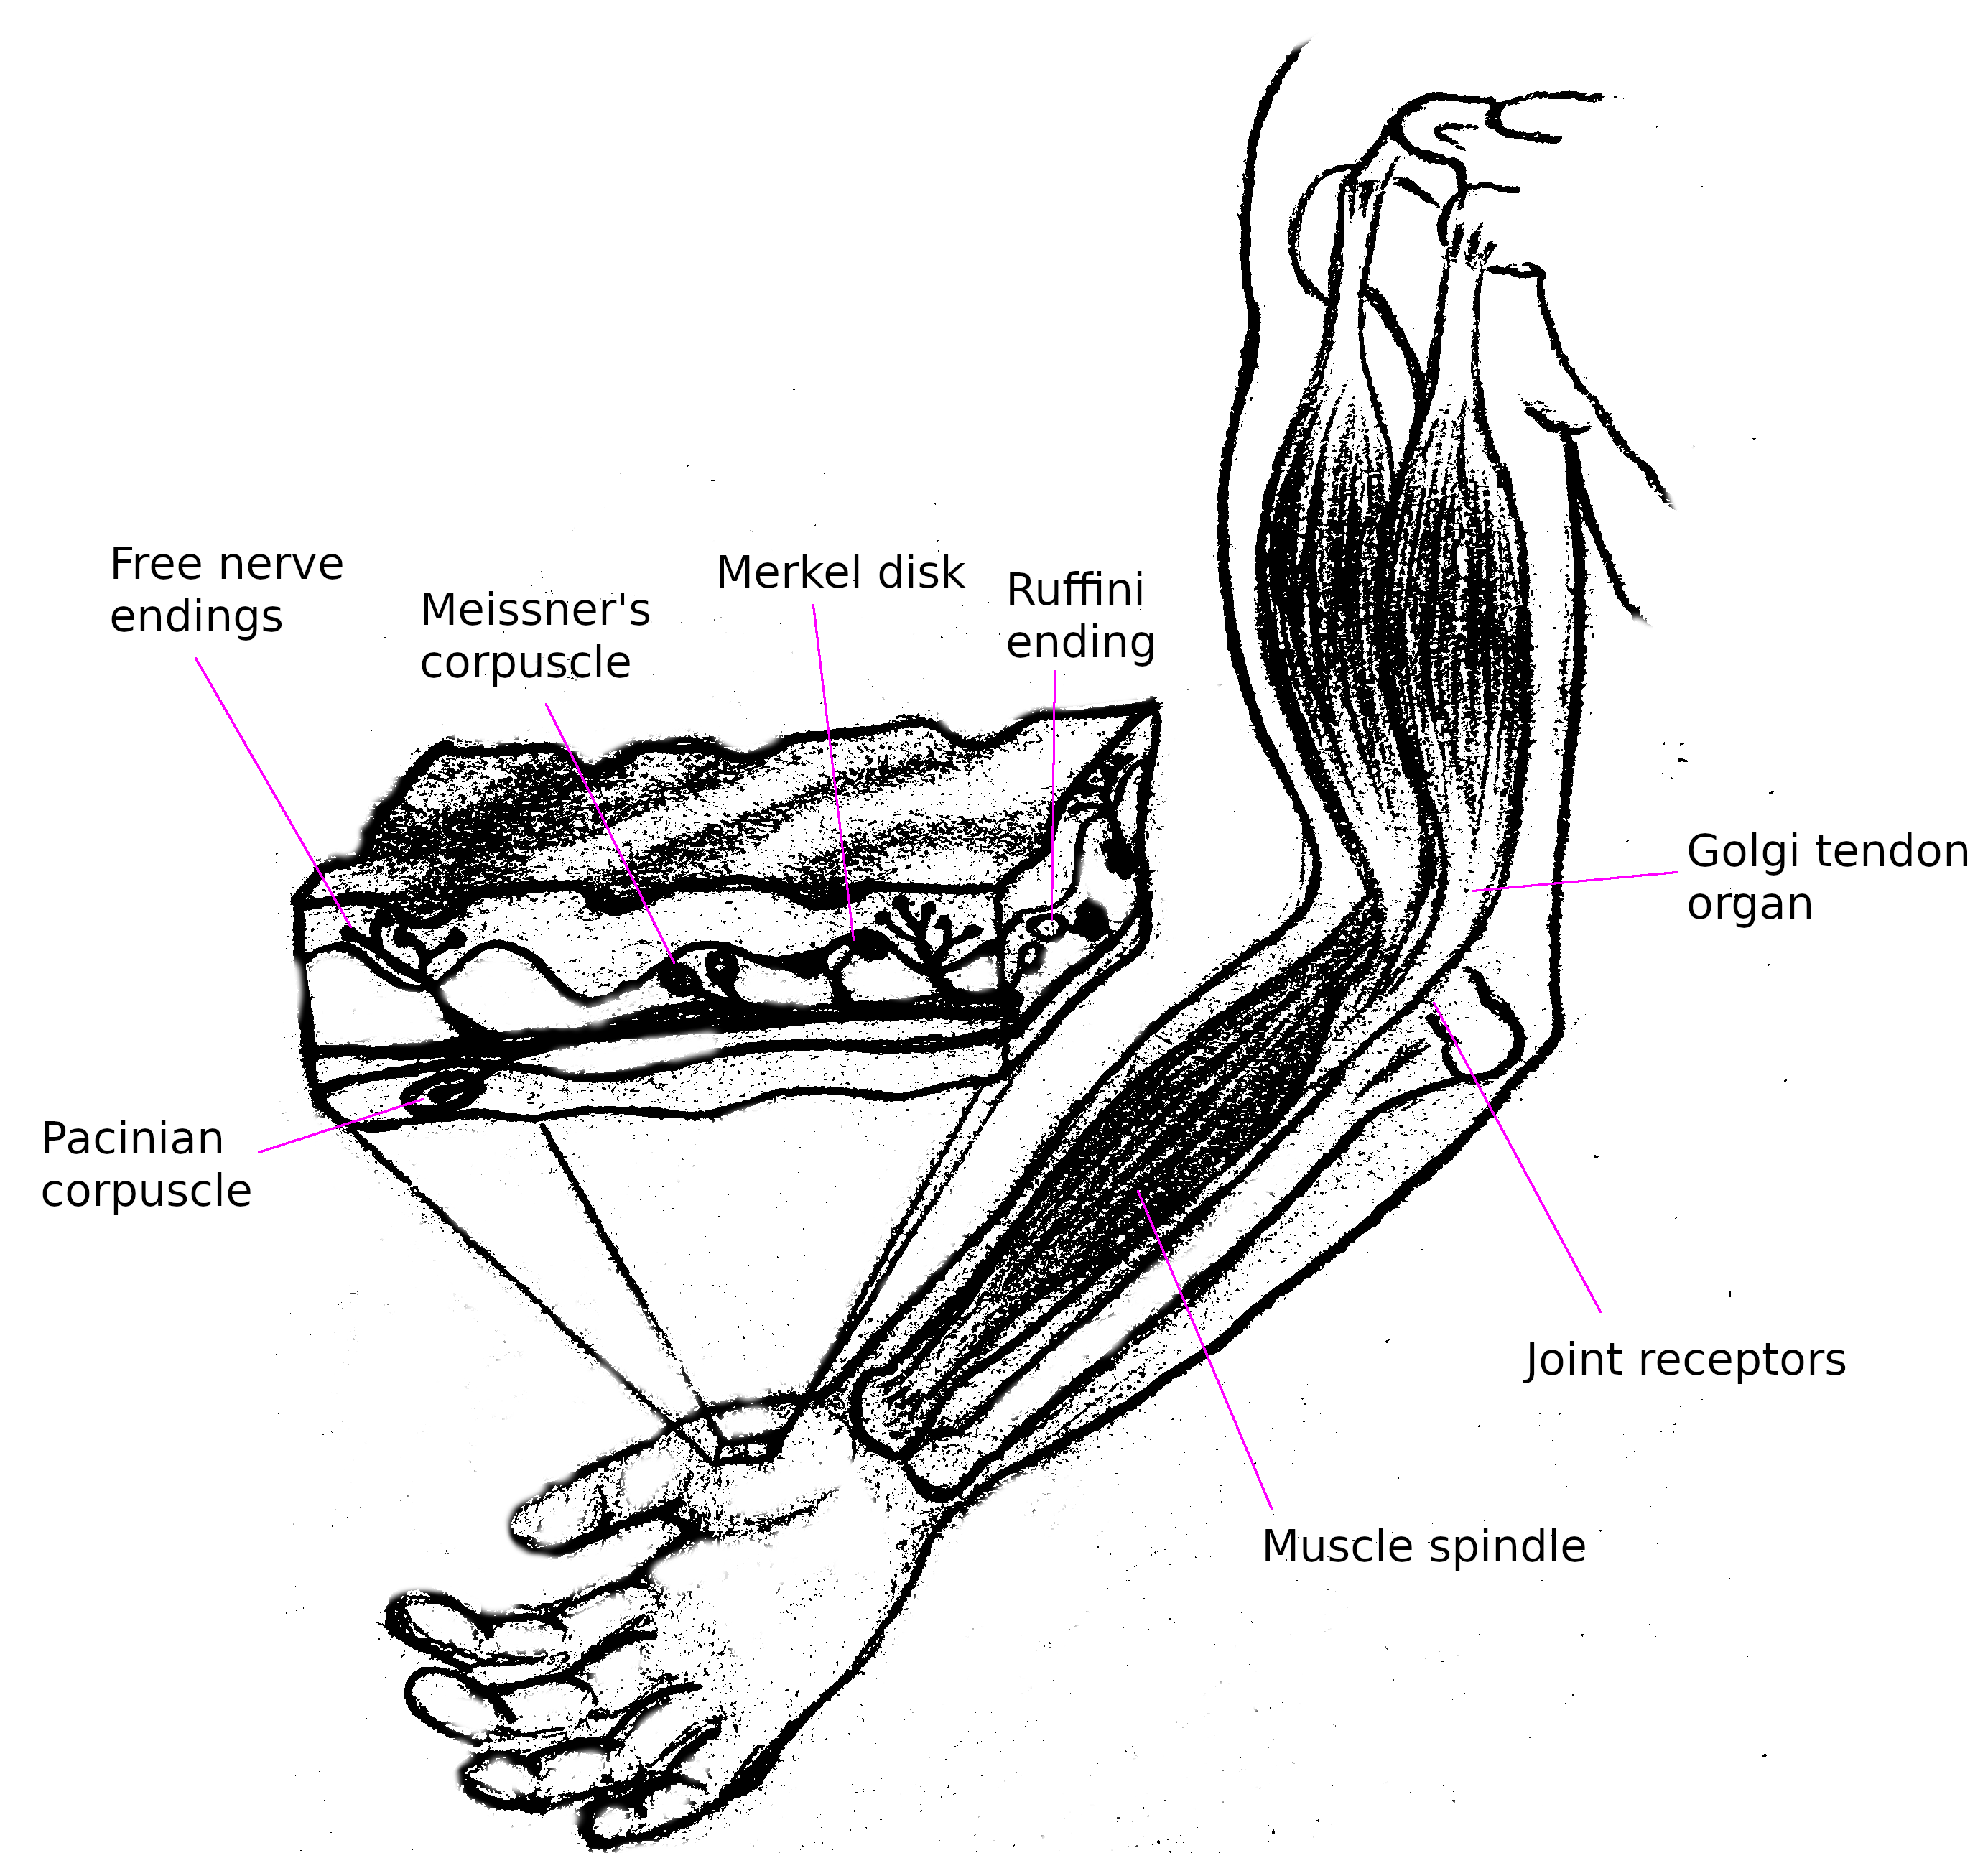
\includegraphics[width=0.6\linewidth]{Figures/propriocetors_n_cutaneous_mechanoreceptors_labelled.png}
    \caption{Examples of the locations of proprioceptors and cutaneous mechanoreceptors in the human body.}
    \label{fig:proprioceptors-mechanoreceptors}
\end{figure}

The function of both kinds of receptor have been mimicked by certain device technologies. For example, proprioceptors have been mimicked in wearables and human assistive devices where joint motion has been estimated by rigid sensors such as rotary/linear encoders, inertial measurement units (IMUs), and soft stretch sensors; both rigid and stretchable sensors have been fixed adjacent to joints to calculate pose estimates of limbs \cite{OBrien2014,Eguchi2020,Chatfield2021,Kim2022}. The rigid sensors can be higher resolution but are often bulky and don't accurately represent the deformation undergone by the human limbs. Soft flexible sensing alternatives are scarce but do not constrain the natural limb motion. However, optical motion capture systems can accurately map un-occluded limbs with high accuracy without encumbering the subject. Examples of such devices are displayed in Figure \ref{fig:proprio-tech}. 
%% Todo: Get copyright permission from image owners %%
\begin{figure}[H]
    \centering
    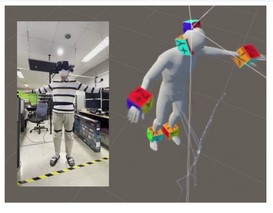
\includegraphics[width=0.4\linewidth]{Figures/imu-pose-tracker-kim2022.jpg} % no copyright permission required
    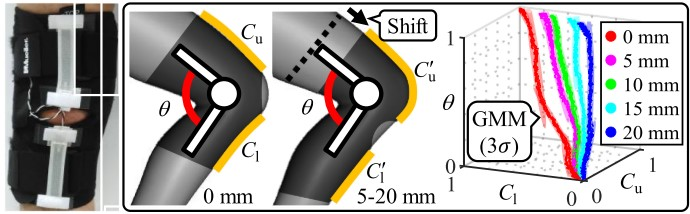
\includegraphics[width=0.4\linewidth]{Figures/knee-stretch-sense-eguchi2020.jpg} % 
    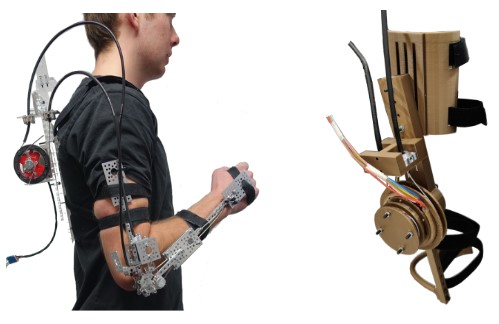
\includegraphics[width=0.4\linewidth]{Figures/logan-assitive-arm-device.jpg}
    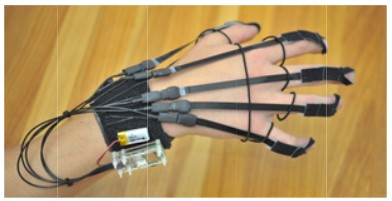
\includegraphics[width=0.4\linewidth]{Figures/stretch-sense-OBrien2014.jpg}
    \caption{Clockwise from top left: IMU pose estimation \cite{Kim2022} ($\copyright$ 2022 MDPI), stretch sensor knee joint pose estimation \cite{Eguchi2020} ($\copyright$ 2020 IEEE), encoder elbow pose joint estimation \cite{Chatfield2021}, stretch sensor hand joint pose estimations \cite{OBrien2014}.}
    \label{fig:proprio-tech}
\end{figure}

\subsection{Skin Construction and Types}
Skin is a laminate structure consisting of three main layers, the epidermis, dermis, and hypodermis. The top two layers the epidermis and dermis are a subset of the cutaneous layer which contain the majority of the pressure-sensitive mechanoreceptors \cite{McGrath2010}.

The skin can be categorised as glabrous/hairless or non-glabrous/hairy. Glabrous skin contains many of the mechanoreceptors given in Figure \ref{fig:proprioceptors-mechanoreceptors} whereas non-glabrous skin will also contain C-tactile afferent receptors for obtaining sensations through hair follicles. However this work is exploring simple monolithic/homogeneous-composite bodies so will not be replicating the sensor function of non-glabrous skin.

Depending on the region of skin different force resolution and spatial resolution will incur. Relevant cutaneous mechanoreceptors and their functions are given in Table \ref{tab:mechanoreceptors-table}. The tensile properties of skin is governed by skin tension lines, also called Lager's lines, which show the direction in which the maximal stretch can occur. 

%\begin{table}[H]
%    \centering
%    \caption{Comparison of typical mammalian mechanoreceptors characteristics \cite{Roudaut2012}.}
%    \label{tab:mechanoreceptors-table}
%    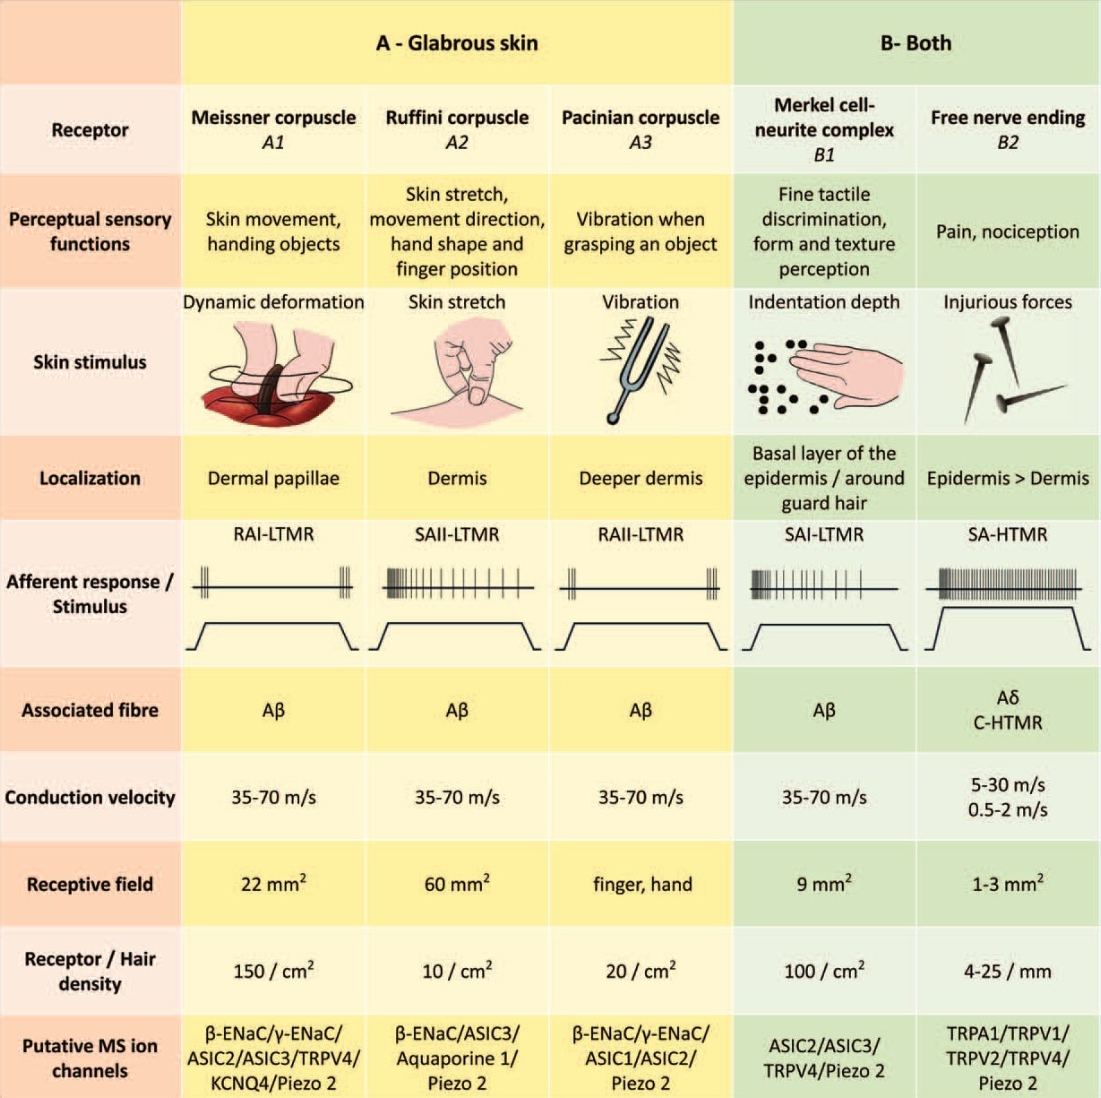
\includegraphics[width=9cm]{Figures/mechanoreceptors-table-cropped.jpg}
%\end{table}
\begin{table}[H]
    \centering
	\caption{Comparison of typical mammalian mechanoreceptor characteristics \cite{Roudaut2012}.}
	\label{tab:mechanoreceptors-table}
	\begin{tabular}{|p{0.24\linewidth}|p{0.21\linewidth}|p{0.21\linewidth}|p{0.21\linewidth}|} \hline
		\textbf{Mechanoreceptor} & Meissner corpuscle A1 & Ruffini Corpuscle A2 & Pancian Corpuscle B1 \\ \hline
		\textbf{Perceptual   sensory functions} & Skin movement, handling objects & Skin stretch, movement direction,   hand shape, and finger position & Fine tactile discrimination, form   and texture perception \\ \hline
		\textbf{Skin stimulus} & Dynamic deformation & Skin stretch & Indentation depth \\ \hline
		\textbf{Localisation} & Dermal papillae & Dermis & Basal layer of epidermis / around   guard hair \\ \hline
		\textbf{Conduction velocity} & 35 - 70 m/s & 35 - 70 m/s & 35 - 70 m/s  \\ \hline
		\textbf{Receptive field} & 22 mm$^2$ & 60 mm$^2$ & 9 mm$^2$ \\ \hline
		\textbf{Receptor density} & 150 / cm$^2$ & 10 / cm$^2$ & 100 / cm$^2$ \\ \hline
	\end{tabular}
\end{table}
%% Todo: Get copyright permission from image owners


\subsection{Characterising skin}
\label{subsec:Characterising skin}
The sensing qualities of skin is crucial for the sensory feedback in complex manipulation tasks. To aid the creations of technology that mimics qualities of biological pressure sensitive skin, the mechanical properties of must be characterised. Similar to soft/flexible sensor technology, biological human skin is highly variable in terms of its mechanical and sensing properties depending on the region of skin, giving large variation in skin characteristics. To match or supersede the function of human skin soft sensing technology must be configurable in terms of their mechanical characteristics. Skin can be characterised in terms of the following mechanical characteristics:
\begin{itemize}
    \item Elastic modulus -  The static elastic properties determined by a linear region of stress and strain of the material. [Pa]
    \item Storage and loss modulus - The dynamic elastic and viscoelastic properties determining the relationship between stress and strain. [Pa]
    \item Ultimate tensile stress (UTS) - The maximum tensile stress that a material can tolerate before breaking [Pa]
    \item Life cycle - The time or number of actuation cycles in which it takes for the actuator to degrade such that it cannot perform its intended purpose to specified standards.
    \item Viscoelastic creep and relaxation - All viscoelastic materials will experience strain creep and stress relaxation to varying degrees depending on the viscoelastic properties of the material. [mm.s$^{-1}$ and s]
    \item Skin thicknesses - the thickness of all layers of skin the cutaneous epidermis and dermis and thickness of the hypodermis. [mm]
    \item Skin surface area - Biological skin has a large surface area and can also be regionalised to map skin function and sensitivity. [m$^2$]
    \item Isotropy/Anisotropy - The directionality of skin properties, also known as skin tension lines, give a topological map of the maximal stretch (i.e. minimal elastic modulus) direction of regions of skin.
\end{itemize}
Some of the functional properties in terms of pressure mapping include:
\begin{itemize}
    \item Spatial resolution and touch acuity - The spatial resolution of biological skin, which is mainly dependent on the innervation, mechanoreceptors density, and thickness of the cutaneous layers of skin \cite{Landry2021,Klein2016,Krotoski1993}.
    \item Static force resolution - This is the detection resolution of static or slow-acting forces acting upon the skin \cite{Krotoski1993}.
    \item Temporal resolution - This is the detection resolution of fast-acting forces acting upon the skin often required for texture recognition \cite{Landry2021,Krotoski1993}.
\end{itemize}

A quantitative characterisation of mechanical and pressure sensing functional skin properties include:
\begin{itemize}
    \item Elastic modulus -  varies largely depending on test method, test skin type, and subject. Values found in literature include 83.3 ± 34.9 MPa \cite{Annaidh2012}, 0.1 - 2.4 MPa \cite{Khaothong2010}, and 10.4 - 89.4 kPa \cite{Zheng1999}.
    \item Storage and loss modulus - varies largely depending on test method, test skin type, and subject. Values found in literature range include 141.9 ± 34.8 Pa and 473.9 ± 42.5 Pa at 0.8 Hz \cite{Holt2008}, 473.9 ± 42.5 Pa and 32.3 ± 10.0 Pa at 205 Hz \cite{Parvini2022}.
    \item Ultimate tensile stress - Two studies showed comparable results of 21.6 ± 8.4 MPa \cite{Annaidh2012} and 28.0 ± 5.7 MPa \cite{Ottenio2015}.
    \item Life cycle - Skin cells are constantly growing, dying, and shedding. Skin is always actively remodelling based on external stimuli \cite{McGrath2010}.
    \item Strain creep - The strain creep was found to be 2.7 kPa.s for a 10 Pa step input on a dermis skin sample \cite{Holt2008}.
    \item Skin thicknesses - The thickness of human cutaneous skin ranges from 0.6 to 2.6 mm with an average skin thickness of 2 mm \cite{Landry2021}.
    \item Skin surface area - The average surface area of skin in adult humans is 1.7 $\pm$ 0.1 m$^2$ \cite{Landry2021}.
    \item Isotropy/Anisotropy - The tension lines in skin are determined by collagen fibre orientation and dynamic stretch events \cite{Paul2018}. The elastic modulus of human skin was reported to be 160.8 ± 53.2 MPa parallel to the skin tension lines and 70.6 ± 59.5 MPa perpendicular to the tension lines \cite{Ottenio2015}. The UTS of human skin was reported to be 28.0 ± 5.7 MPa parallel to the tension lines and 15.6 ± 5.2 MPa perpendicular to the tension lines \cite{Ottenio2015}.    
\end{itemize}
Some common metrics used in the biomedical field include:
\begin{itemize}
    \item Spatial resolution and touch acuity - The tactile field area increases with indentation depth for certain mechanoreceptors with a range of 5 - 12.6 mm$^2$ \cite{Deflorio2022}. Two point discrimination is another metric for determining spatial resolution an has been determined as 3.7 ± 0.7 mm \cite{Yokota2020}. The receptive field varies depending on the mechanoreceptors used so has been reported to be between 1 and 60 mm$^2$ as another methods of inferring spatial resolution \cite{Roudaut2012}.
    \item Force resolution - Minimum force detection on various regions of human skin was found to be between 67 - 1007 mg \cite{Ackerley2014}, and fast and slow acting  mechanoreceptors 0.73 - 122.6 mN \cite{Strzalkowski2015}.
    \item Temporal resolution - Depending on the mechanoreceptors utilised, a frequency range of 0 to 800 Hz can be perceived by human skin \cite{Deflorio2022}
\end{itemize}


\subsection{Skin Modelling}
% the point of this section is to show that skin is complex to model mechanically and why. Then we can talk about how our composite compares. 
Developing robust mechanical models for human skin is non-trivial for three main reasons:
\begin{enumerate}
    \item High degree of viscoelasticity
    \item Self-regeneration and healing
    \item Constructed from various types of cells in a laminate structure 
\end{enumerate}
To solve the complexity of modelling such a material a review by Landry et al. \cite{Landry2021} shows that many researchers have applied various non-linear mechanical models including Ogden, Mooney–Rivlin, Neo-Hookean, Yeoh, Humphrey, and Veronda–Westmann. When recreating an artificial muscle it is desirable to minimise the mechanical material model complexity so that the material can be more easily integrated into a control system with known behaviour. Similar modelling techniques can be used to model conductive particle elastomer composites due to the similar hyper-elastic and viscoelastic behaviours observed.



\section{Artificial Sensing - Pressure Mapping Technology}
% Artificial skin review
% Give the range of technologies available expand upon review given in Pt II EIT sensor paper.
This section outlines some of the main technologies which are flexible and/or soft a comparable softness to human skin tissue and can map force events throughout a surface.
Through comparison of various materials EAPs have shown many similarities in mechanical properties to biological skin, identifying EAPs as a promising material for further use in sensor and actuator devices. A particular focus on electroactive polymer (EAP) based sensing is present due to the potential of miniaturising the technology and the range of miniaturised electronics currently available. EAPs are polymer materials which can be used as transducers that change electrical properties based on a mechanical input, and vice-versa.

% Why does this section matter? How does it link to my research goals? What is it adding to the greater research pool? A large part of my research was looking into making an 'artificial skin sensor'. It has been requested by several reviewers of my journal article to look at state of the art devices similar to mine, from 2020 onwards and for variant of EIT sensing especially. 
Pressure mapping devices can be categorised into their various sensing technology, such as resistive, capacitive, inductive, magnetic, optical, and acoustic. Transduction methods have been compared by Tiwana et al. \cite{Tiwana2012}, with recommendations to pursue `capacitive, resistive, piezoelectric, piezoresistive or a combination' of methods to replicate mechanoreceptors in the human skin. However, additional optical and magnetic/inductive methods will also be considered in the following sections.

Pressure mapping is widely used for many applications including sports equipment grip analysis, foot pressure in gait analysis, in production line part alignment, hospital patient bed and chair pressure injury mitigation, headphone pressure analysis, among many others. These applications are useful for increasing quality of life, optimising sporting performance, object detection, and production efficiency optimisation.

Cutaneous mechanoreceptors have been mimicked by the development of pressure mapping of flexible surfaces. Examples of such technologies include, foot pressure based gait analysis, wheelchair seat pressure mapping. Commercially available examples of these sensors are shown in Figure \ref{fig:mechano-tech}.
\begin{figure}[H]
	\centering
	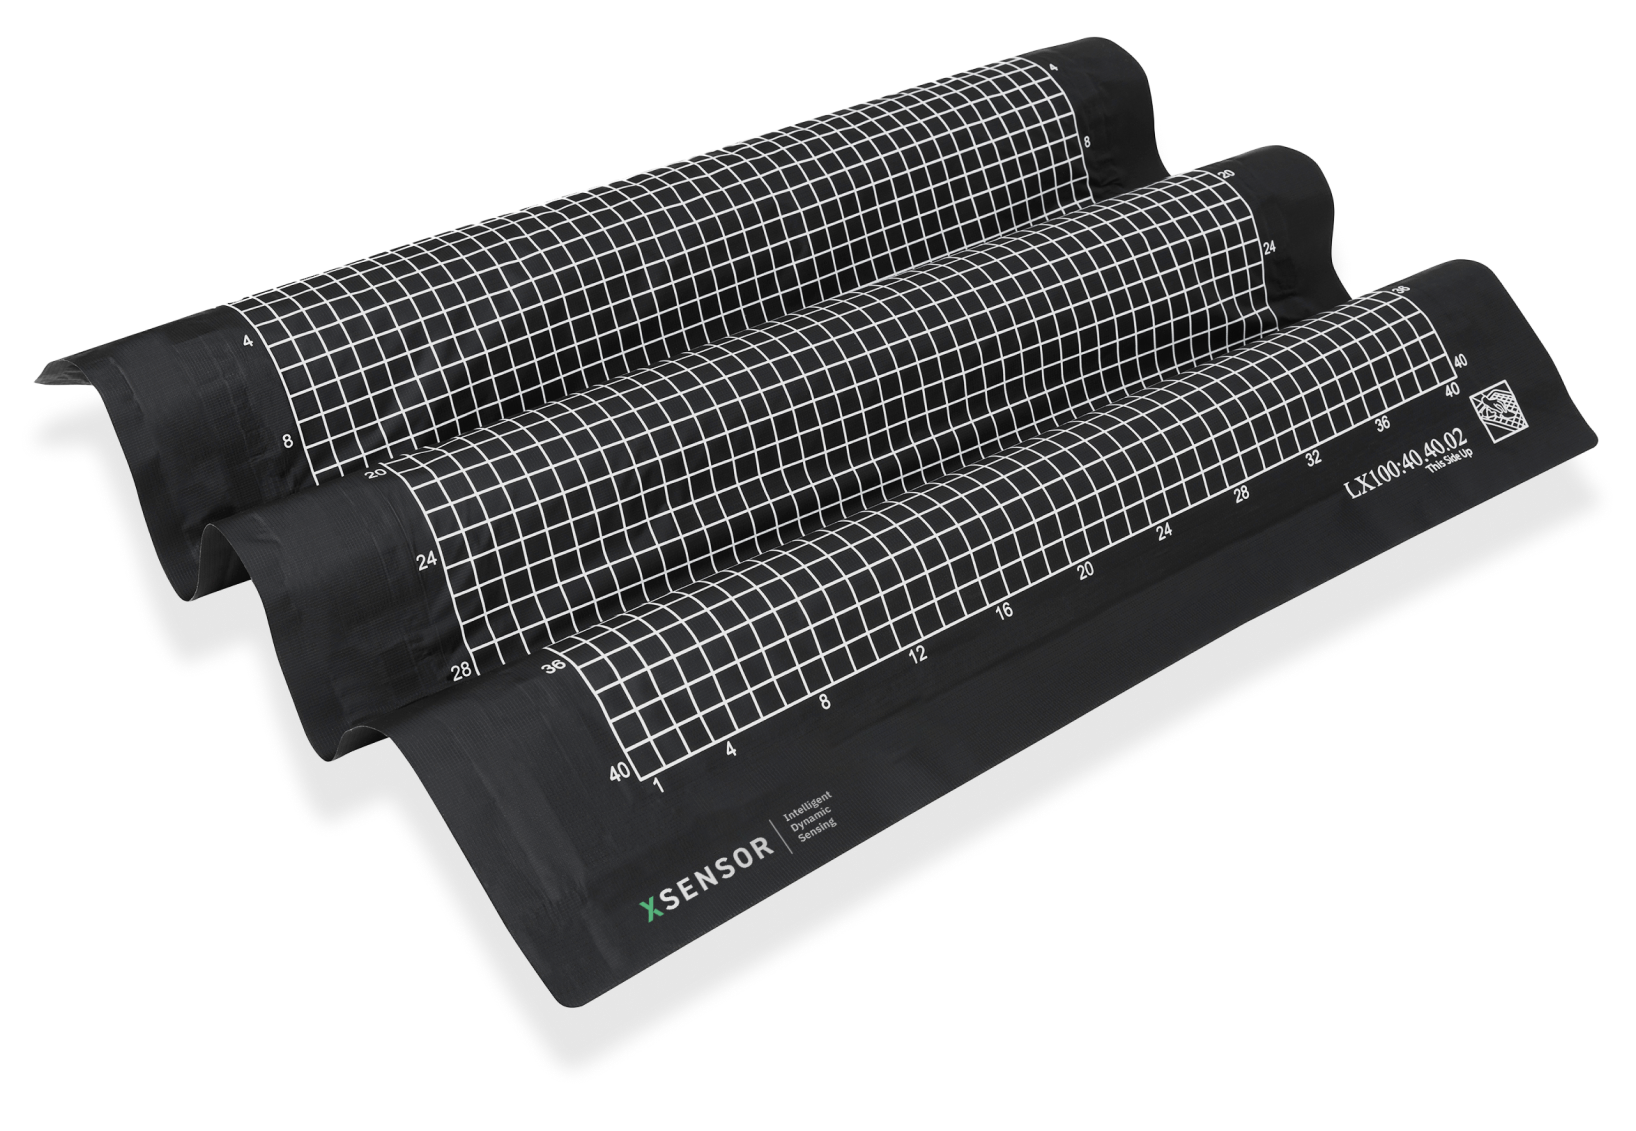
\includegraphics[width=0.4\linewidth]{Figures/xsensor.png}
	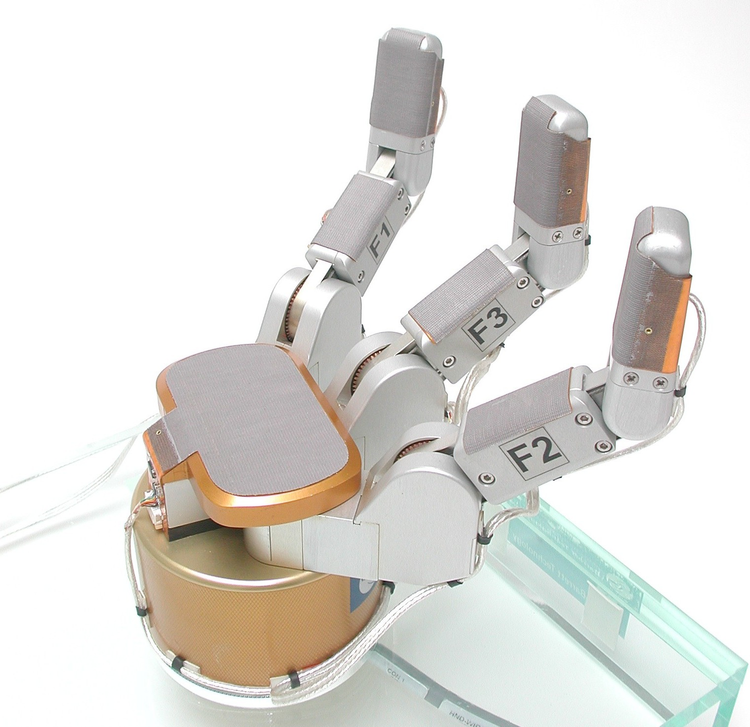
\includegraphics[width=0.4\linewidth]{Figures/Robotic+arm+with+PPS+sensors.png}
	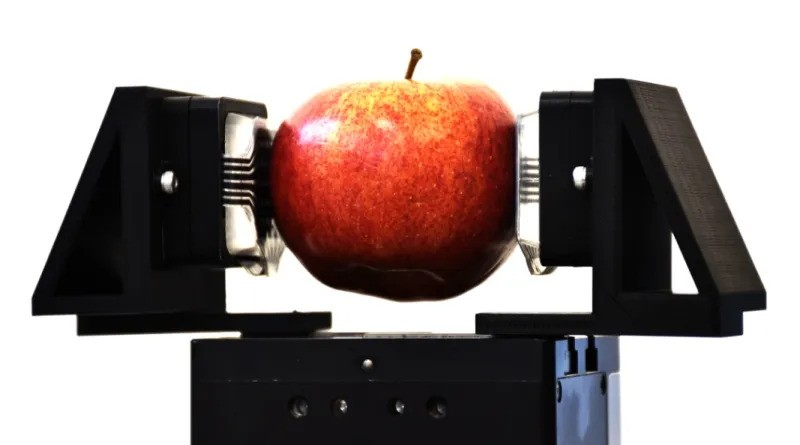
\includegraphics[width=0.4\linewidth]{Figures/powerOn_gripper_apple.jpg}
	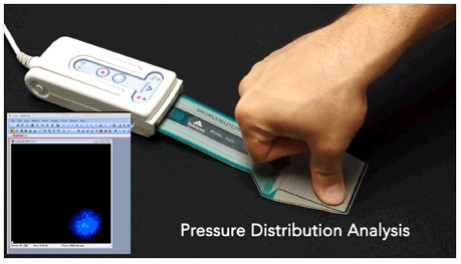
\includegraphics[width=0.4\linewidth]{Figures/tekscan-pressure-sensor.jpg} % only commercial image without permission granted.
	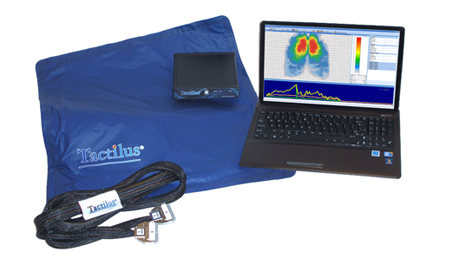
\includegraphics[width=0.4\linewidth]{Figures/tactilus-pressuremap-sensor-laptop.jpg}
	\caption{Various pressure mapping devices. From top-left then clockwise: Xsensor wheelchair pressure mapping sheet ($\copyright$ 2024 XSENSOR\textsuperscript{\textregistered} Technology) \cite{Xsensor}, Pressure Profile Systems pressure sensors on a robotic hand ($\copyright$ 2023 PPS UK limited) \cite{PressureProfile2023}, Soft pressure mapping gripper($\copyright$ 2023 PowerON) \cite{PowerOn}, Tekscan thin pressure mapping platform \cite{Tekscan}($\copyright$ 2024 Tekscan Inc.), Tactilus seat pressure mapping system \cite{SensorProducts}($\copyright$ 2024 Sensor Products Inc.)}
	
	\label{fig:mechano-tech}
\end{figure}
%% Todo: Get copyright permission from image owners %%
Many of these pressure mapping technologies don't accurately mimic desirable qualities of regular biological skin and are specialised for their specific use cases.


\subsection{Capacitive}
Similar to resistive pressure mapping, capacitive pressure mapping has more commonly been done using arrays of capacitive elements. The operating principle of capacitive-based strain sensors rely on the deformation of sensel capacitors comprising of a dielectric elastomer and electrodes \cite{Sapra2023,Zhu2021,Liang2015}.
\begin{figure}[H]
	\centering
	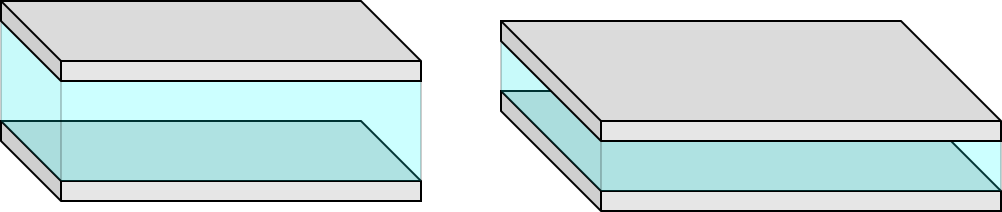
\includegraphics[width=0.6\linewidth]{Figures/cap_deformed_states_x2_crop.png}
	\caption{A sensel with grey electrodes across a blue dielectric medium. Left: Uncompressed state. Right: Compressed state}
	\label{fig:cap_deformed_cube}
\end{figure}
A pressure mapping sensor can be formed by making an array of the sensel shown in Figure \ref{fig:cap_deformed_cube} an attaching capacitive sensing electronics. To sense a change in capacitance electronics often will use an AC source to determine the phase change due to the change in capacitance and/or using the time constant formed by the changing sensing capacitance.


\subsection{Magnetic}
Magnetic strain mapping devices can be achieved using several methods. One method is to have a three layer stack with Hall effect sensors \cite{Yan2021,Yan2022}. The stack is made up of a the bottom layer full of rigidly connected three dimensional Hall effect sensors, the second layer is made from an elastomer, and the top layer has a magnetic particle unit placed at a set distance above each of the Hall effect sensors. The movement of the magnets alters the magnitude and direction of magnetic field sensed and data can be interpolated to create a map of strain deformation, as shown in Figure \ref{fig:mag_pressure_map_sensor}. 
\begin{figure}[H]
	\centering
	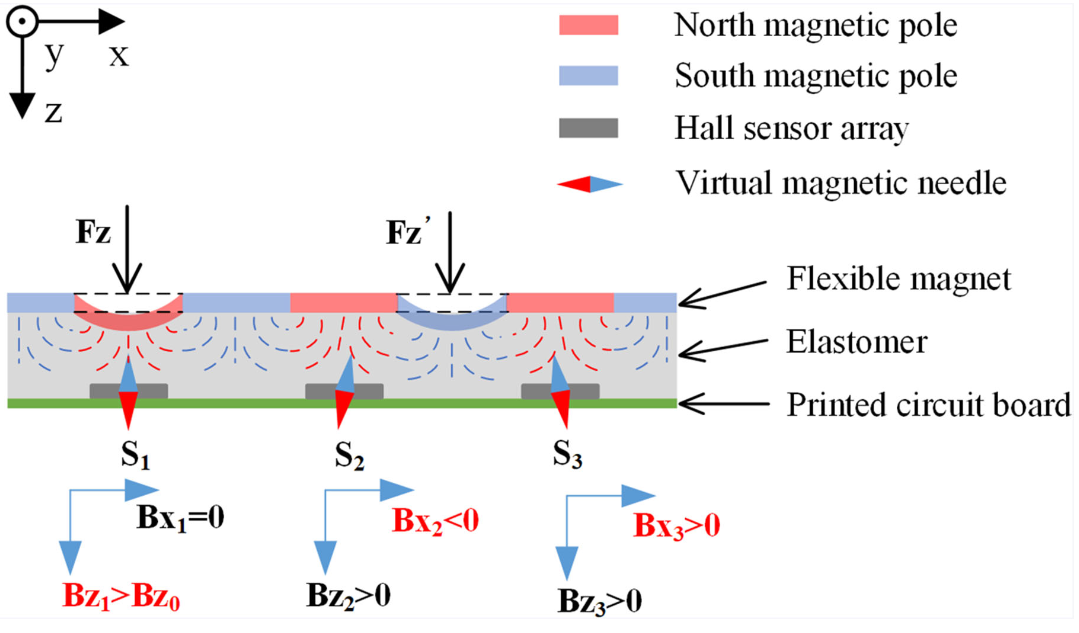
\includegraphics[width=0.6\linewidth]{Figures/mag_pressure_mapping.png}
	\caption{Example of a magnetically-based pressure mapping system designed by Yan et al. \cite{Yan2022} ($\copyright$ 2022 IEEE).}
	\label{fig:mag_pressure_map_sensor}
\end{figure}
The main advantages of this method is that each hall sensor can detect in three dimensions, hence normal and shear forces can be detected, and using magnetism for sensing means less electrical noise in the system. The main disadvantages of this method of sensing is the added complexity in scaling the system and the electronics required and the rigid surface required.  

\subsection{Optical}
There are various methods for making a optically driven artificial skins. A recent review has been curated by Lee et al. \cite{Lee2023} all of the different methods of using optics for creating tactile sensors. The main advantages of optical sensors include the high speed sensor response, immunity to electrical noise, and their non-invasive nature. The main disadvantages include, the bulky hardware required for driving the optics and signal processing, the potential interference of external light sources, and the materials that can carry optical signals. An example application of an optically-based soft pressure mapping sensor is provided in Figure \ref{fig:optical_soft_mapping}.
\begin{figure}[H]
	\centering
	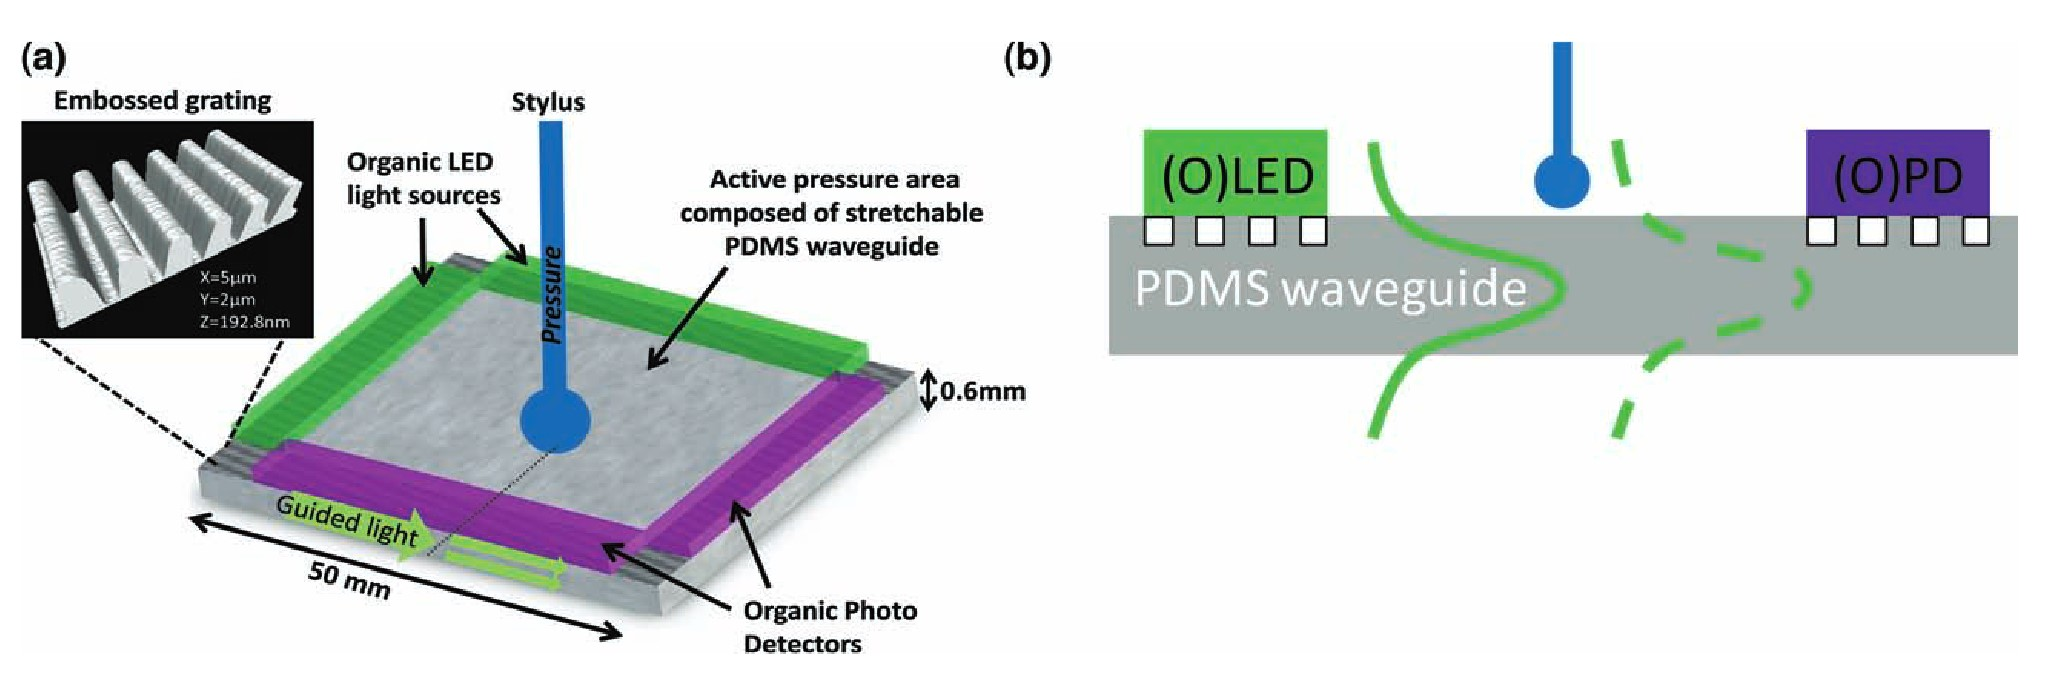
\includegraphics[width=0.75\linewidth]{Figures/optical_soft_pressure_mapping.jpg}
	\caption{Example optical pressure mapping sensor using a planar PDMS waveguides. a) Schematic of the two-directional stretchable optical pressure sensor. The active	pressure area is comprised of PDMS. b) A cross section view of the optical pressure sensor ($\copyright$ 2012 Wiley) \cite{Ramuz2012}.}
	\label{fig:optical_soft_mapping}
\end{figure}

\subsection{Acoustic}
Acoustic soft tactile sensing has not been explored much compared to the other forms of sensing given. Park et al., Hughes and Correll \cite{Park2022,Hughes2015} have created a system which uses passive acoustic tomography (PAT) to localise and and classify different types of touch. This form of tactile sensing is the most similar to the biological system of mechanoreceptors which are specialised to detect certain frequencies of vibration.


\subsection{Resistive}
Soft resistive pressure mapping has been commonly achieved in the past by using arrays of piezoresistive sensor elements, some of which are shown in Table \ref{tab:non_eit_sensor_compare}. The resistive elements can be made using several different flexible piezoresistive materials, such as conductive particle polymer composites \cite{Sun2020,Lu2014,Spahr2017}, intrinsically conductive polymers \cite{Lu2014,Hazelton2023,Mukherjee2023}, microfluidic metals \cite{Park2010,Jung2015,Kim2019}, hydrogel structures \cite{Yuk2016,Park2022,Chen2023}, and flexible piezoresistive semiconductors \cite{Xu2023,Sim2019}.

\begin{table}[H]
	\centering
	\caption{Comparison of different potential piezoresistive sensor materials. Rated 1 to 5, where 1 is low and 5 is high.}
	\label{tab:comparing-piezo-r-materials}
	\vspace{3cm}
	\begin{tabular}{|p{5cm}|p{1cm}|p{1cm}|p{1cm}|p{1cm}|p{1cm}|p{1cm}|p{1cm}|p{1cm}|}
		\multicolumn{1}{l}{\textbf{Material:}} & \multicolumn{1}{c}{\begin{rotate}{60} \hspace{0.1cm}\vspace{-2cm} \textbf{Conductivity} \end{rotate}} & 
		\multicolumn{1}{c}{\begin{rotate}{60} \hspace{0.2cm}\vspace{-2cm} \textbf{Piezoresistivity} \end{rotate}} & 
		\multicolumn{1}{c}{\begin{rotate}{60} \hspace{0.2cm}\vspace{-2cm} \textbf{Softness} \end{rotate}} & 
		\multicolumn{1}{c}{\begin{rotate}{60} \hspace{0.2cm}\vspace{-2cm} \textbf{Manufacturability} \end{rotate}} & 
		%			\multicolumn{1}{c}{\begin{rotate}{60} \hspace{0.2cm}\vspace{-2cm} \textbf{Cost} \end{rotate}} & 
		\multicolumn{1}{c}{\begin{rotate}{60} \hspace{0.2cm}\vspace{-2cm} \textbf{Durability} \end{rotate}} & 
		\multicolumn{1}{c}{\begin{rotate}{60} \hspace{0.2cm}\vspace{-2cm} \textbf{Toxicity} \end{rotate}} \\ \hline
		
		Conducting polymer \cite{Guo2018,Hazelton2023,Bhattacharjee2020,Mukherjee2023} & 2 & 2 & 1 & 2 & 3 & 3 \\ \hline
		Electrolytic hydrogel \cite{Guo2018,Shen2022,Li2020a,Li2020b,Lu2014,Wang2018} & 3 & 4 & 5 & 3 & 2 & 3   \\ \hline
		Conductive particle paste / liquid metal \cite{Chen2020a,Park2010,Jung2015} & 5 & 2 & 4 & 2 & 2 & 2 \\ \hline
		Conductive textile / fabric \cite{Jeong2020a,Yao2012,Rashid2022} & 4 & 4 & 4 & 2 & 5 & 4  \\ \hline
		Conductive particle polymer \cite{Princy1998,Spahr2017,Duan2014,Buketov2020} & 3 & 5 & 4 & 4 & 4 & 4 \\ \hline
	\end{tabular}
\end{table}

Conducting polymers, also known as intrinsically conducting polymers (ICPs), were discovered and developed by Shirakawa et al. \cite{Shirakawa1977} in 1977. ICPs are doped to change their electron band structure to allow for electrical conduction, however are very difficult to fabricate and not durable due to their water solubility. Electrolytic hydrogels are a hydrogel which have absorbed a electrolytic fluid. The electrolytic fluid provides a conductive through the material, however it can be temperature sensitive, due to electrolyte solution evaporation and the changing mechanical properties. Conductive particle paste and liquid metals, often have high conductivity, but can be difficult to fabricate with due to their fluid state. Conductive fabrics and textiles are often used to block EMI and have often comprise a  2D weave of conductive fibres requiring several steps to manufacture. Conductive particle polymers are similar to conductive particle paste, however can be made of varying polymers drastically altering the mechanical storage and loss moduli. This allows for a range of elasticity and stiffness in the material and increased piezoresistivity, making conductive particle polymers a promising material for further development of artificial skin and muscle technology. 


\subsection{Soft Pressure mapping technology comparison}
To improve upon existing pressure mapping technology and ensure novelty, the state-of-the-art technologies are compared. There have been a range of works investigating sensors with a range of softness' and performance. A comparison of these start-of-the-art soft pressure mapping sensor works is given in Table \ref{tab:non_eit_sensor_compare}.  The range of softnesses and seen in this comparison is comparable to that mentioned in Section \ref{subsec:Characterising skin}. However other the characteristics such as durability, reliability, biocompatibility, topology, and resolution of each sensor technology cannot match that of biological human skin.

The main advantage for using EAP based composite materials for pressure mapping sensors over magnetic and optical sensors include the lack of bulky external drive components such as electromagnetics, lasers, and optical detectors. Although capacitive sensors have similarly small bulk for their external drive components compared to resistive sensors, capacitive sensors require more complex layering, which increases the fabrication complexity when scaling into a 2D array of capacitive sensels. 
%%% COMPARISON OF NON-EIT SENSOR EQUIVS %%%
\newgeometry{left=2in,right=0in,bottom=-0.25in,top=0in}
\setstretch{1.0}
\begin{landscape}
		\newcolumntype{L}[1]{>{\raggedright\let\newline\\\arraybackslash\hspace{0pt}}m{#1}}
%		\thispagestyle{plain}
		 \begin{table}[H]
		 	\caption{Comparison of soft pressure mapping sensor technologies. Dashes represent data not present in the related paper.}
		 	\label{tab:non_eit_sensor_compare}
			\begin{tabular}{|L{2.9cm}|L{2.4cm}|L{2.8cm}|L{3cm}|L{3.0cm}|L{2cm}|L{2.4cm}|L{2cm}|L{2.1cm}|} \hline 
				\textbf{1st Author} & \textbf{Sensing principle} & \textbf{Sensing region material} & \textbf{Sensing region elastic modulus or shore hardness} & \textbf{Electrodes per sensing position} & \textbf{Repeatability} & \textbf{Time series data given} & \textbf{Spatial resolution} & \textbf{Temporal resolution} \\ \hline
				Gilanizadehdizaj \citep{Gilanizadehdizaj2022} & Piezoresistive & Ecoflex30-00 rGO sponge & 40 kPa & 2 sensels / electrode & 10 cycles for each stress & \textit{-} & 10 $\times$ 10 mm & - \\ \hline
				Fu \citep{Fu2020} & Piezoresistive & Carbon black silicone composite & 1.5 MPa & 0.625 sensels / electrode & 50000 cycles & Yes. & 12 $\times$ 12 mm & 60 ms \\ \hline
				Yang \citep{Yang2022} & Piezoresistive & Ecoflex graphene sponge & - & 2 sensels / electrode & 800 cycles & Yes. & 10 $\times$ 10 mm & 150 ms \\ \hline
				Liang \citep{Liang2015} & Capacitive & PDMS, PET, Si, SiO$_2$, Cu laminate & 4000 MPa & 1 sensel / electrode & - & Implicitly. & 4 $\times$ 4 mm & - \\ \hline
				Yan \citep{Yan2021,Yan2022} & Magnetic & Ecoflex 00-50 & 83 kPa & 11 IC pins / sensel & 30,000 cycles & Yes. & 0.2 mm & 15 ms \\ \hline
				Rossiter \citep{Rossiter2005} & Optical & Polymer foam & - & 2 sensels / electrode & - & - & 10 $\times$ 10 mm & - \\ \hline
				Shimdera \citep{Shimadera2022} & Optical & Super clear silicone & 40 A & N/A. One fibre optic LASER and   one camera. & Error rose 1.7\% in 30 days & Yes. & approx. 20 $\times$ 20 mm / 0 - 1100 um & Sample rate 1.6s. \\ \hline
				Ramuz \citep{Ramuz2012} & Optical & PDMS & - & N/A. Two arrays of OLEDs and Detectors used. & 900 cycles & Yes. & Not localised. & 300 ms \\ \hline
			\end{tabular}
		\end{table}
\end{landscape}
\newgeometry{left=2in,right=0in,bottom=0in,top=2in}
\setstretch{1.5}

%% LEAVE THIS LIT REVIEW AS BACKGROUND IN THE RELEVANT CHAPTERS??
% \subsection{Electrical Impedance Tomography}
%% % How does EIT work
%
% \subsection{Electric Field Imaging}
% % Quick review on the theoyr of EFT and how it differs from EIT. Discuss it's importance and reference how this work looks towards using capacitive shunting AND EIT to create a faster EIT-based pressure mapping sensor.
%
% \subsection{EIT-based Skins}
%% % Give a review on the state of art EIT-based skin technology


\section{Bio-Actuation - Muscle Form and Function}
% lit review on 'An engineering perspective on the function of human muscle'
%\textit{Note: This section was taken from literature reviews from 3 years ago, when I was going to research DEAs. Needs a re-review ASAP.}

Biological muscles are a product of millions of years of evolution and the motion and other mechanical characteristics of biological structures is yet to be outperformed by artificial muscle technology. To determine how to quantify the performance of a biological muscle this section gives foundational knowledge about muscle function, structure, and how it can be characterised from an engineering perspective rather than the typical biological perspective, so that similar actuator devices with similar attributes can then be investigated.

Biological muscle is a naturally occurring tissue comprised of muscle fibres bundled together to apply a contractile force on connecting tissue or, in the case of smooth muscle, applying a force on itself. The base actuator units of muscle are proteins myosin and actin filaments, which effectively slide against each other to produce a contractile motion. The root cause of a muscle contraction is an electrochemical signal sent from the central nervous system to a motor neuron/s which travel to the muscle where electrochemical reactions take place for the contraction to occur \cite{Keynes2011}.
\begin{figure}[H]
	\centering
	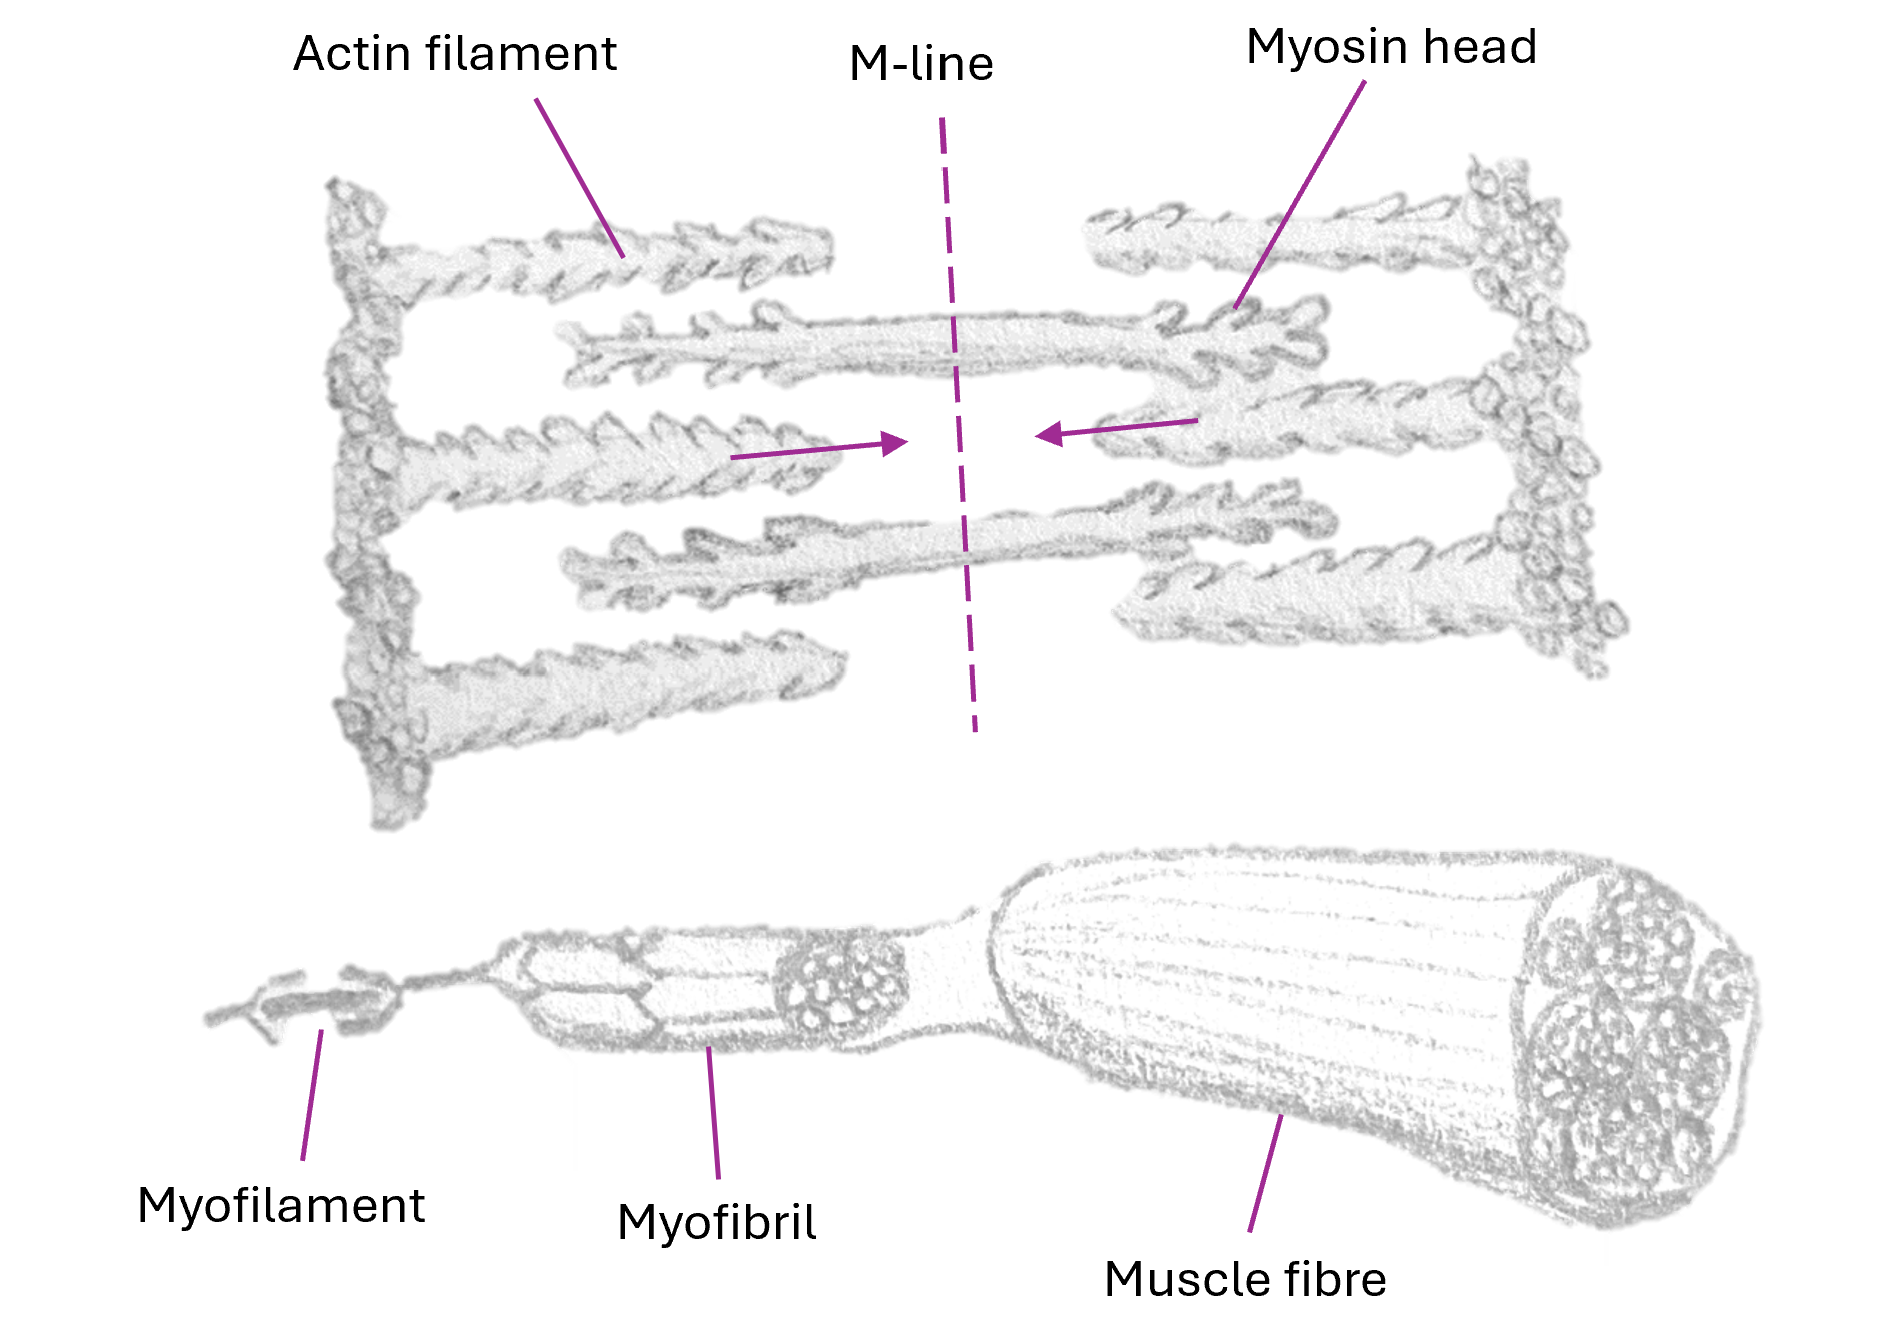
\includegraphics[width=0.6\linewidth]{Figures/motor-unit-myo-fibril-to-fibre.png}
	\caption{Components of a biological muscle contractile unit and meta-structure.}
	\label{fig:muscle_units}
\end{figure}
The sliding motion of the myosin and actin filaments is due myosin heads binding to the actin and pulling the actin towards a middle line (M-line) in multiple stroke actions. These filament actuators are stacked in three dimensions within a muscle fibre to amplify contractile stress and strain as shown in Figure \ref{fig:muscle_units}.

On a macro scale, muscle is made up of bundles of fasicles connected together with a tissue called perimysium. Within the fasicles are many muscle fibres (i.e. muscle cells) which are surrounded by a connective tissue called endomysium. Within the muscle fibres there are many sacromeres stacked within a cylindrical-like structure called a myofibril. Each sacromere contains a contractile unit of myofilaments. 



\subsection{Characterising a muscle}
To quantify the performance of a biological muscle, certain metrics are compared. An artificial and biological muscle can be characterised using typical mechanical material parameters such as:
\begin{enumerate}
    \item Stress - Force that is applied to the normal of the cross section of the muscle through various states of muscle excitation. [$Pa$]
    \item Strain - The muscle change of length due to the stress applied through various states of muscle excitation. [\%]
    \item Elastic modulus - The elasticity determining the relationship between stress and strain for the linear region of the stress strain characteristic curve. [$Pa$]
    \item Actuation voltage - The voltage required to trigger saltatory conduction in a neuron [V]
    \item Energy density - The work done by the muscle per unit volume or mass. [$J.kg^{-1}$]
    \item Power density - The work done by the muscle per unit volume or mass per unit time. [$W.kg^{-1}$]
    \item Ultimate tensile strength - The maximum tensile stress that a material can tolerate before breaking. [$Pa$]
    \item Efficiency - The work done by the muscle compared to the energy put into the system, known as metabolic cost in biological muscles. [\%]
    \item Actuation frequency - The frequency range of actuation cycles using the system's method of excitation. [$Hz$]
    \item Stroke - The maximum displacement an actuator can achieve [$m$]
    \item Life cycle - The time or number of actuation cycles in which it takes for the actuator to degrade such that it cannot perform its intended purpose to specified standards.
%\newline
%\newline
%    As well as the commonly used medical/biological muscle metric:
%\newline
%    \item Maximum isometric contraction force - the maximum force a muscle can apply without changing strain. This is also related to the ratchet-like mechanism and muscle locking where a muscle can apply a much larger force in a static state, as seen in the myosin binding \citep{Cross2006}.

\end{enumerate}
Only the main characteristics of muscle have been described above. If wanting to mimic other qualities of a biological muscle they should be quantified on a case by case basis depending on the artificial muscle technology being investigated. Some of the above biological muscle metrics have been quantified by previous research as seen below:
\begin{itemize}
	\item Actuation voltage - action potential voltage threshold for a muscle resting at -70 mV is -55 mV. With a peak voltage of +30 mV \cite{Filatov2005,Schmidt-Nielsen2002}.
	\item Actuation frequency - action potentials are commonly between 4 - 12Hz \citep{Popovic2004}
    \item Energy density - energy densities ranging from 0.4 - 40 $J.kg^{-1}$ \citep{Alexander1977}.
    \item Power density - power densities ranging from 9 - 284 $W.kg^{-1}$ \citep{Full2004}
    \item Actuation frequency - natural actuation frequencies ranges 1 to 180 $Hz$ \citep{Full2004}.
    \item Strain - ranging from 5 - 30\% \citep{Duduta2019}.
    \item Efficiency - Thermodynamic efficiency of human muscle is typically between 20-35\% \citep{Smith2005}. However other biological muscle has been seen to reach efficiencies of up to 77\% \citep{Smith2005}.
\end{itemize}
    

\subsection{Muscle Mechanics}
A variety of simplified electromechanical muscle models have been developed. Understanding these models is essential for exploring how biomimetic actuators can be applied in assistive soft robotic devices. First, some fundamental biomechanical muscle models will be discussed.

The stress and strain involved in muscle contraction is more complex than uniform materials and is non-linear. The stress and strain of a passive muscle (i.e. contractile units are not producing internal muscle tension) can be modelled with the following equation; 
\begin{equation}
    \frac{d\sigma}{d\varepsilon} =  \alpha.(\sigma+\beta)
\end{equation}
Where $\varepsilon$ \& $\sigma$ are strain and stress respectively. A solution for this is first order ODE is; 
\begin{equation}
    \sigma = \mu e^{\alpha\varepsilon} - \beta
\end{equation}
Where $\mu$ is a free parameter determined empirically. The stress-strain of a passive muscle can be likened to tension being applied yarn. As more strands of the yarn are pulled into tension the stress increases, then as the last strands are brought into tension a maximum stress is reached, until the yield stress is reached. Linear approximations can still be made over regions of elongation depending on accuracy required for application. The stress-strain of an active muscle (i.e. when it is tetanised) is approximated to a piece-wise quadratic function or bell curve. It is important to note that the stress for both active and passive muscle is near zero when the strain is less than 0.4, demonstrating the yarn-like nature of the muscle stress-strain as shown in Figure \ref{fig:muscle-fibre-stress}.
\begin{figure}[H]
  \centering
  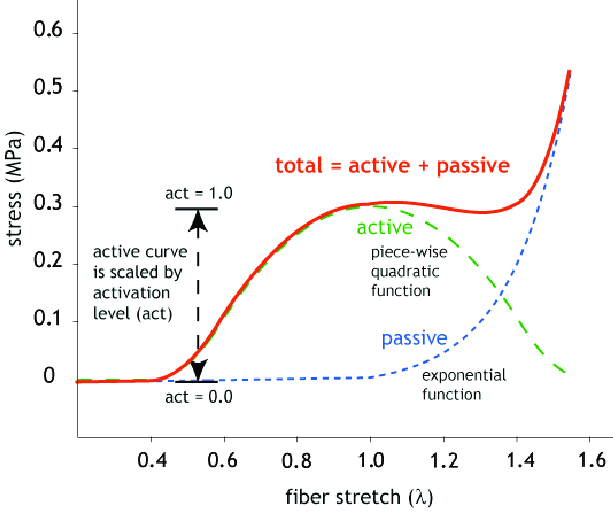
\includegraphics[width=8cm]{Figures/Muscle-fiber-active-and-passive-behavior.png}
  \caption{Stress and strain of active and passive muscles ($\copyright$ J. Teran $|$ ACM 2003) \citep{Teran2003}}
  \label{fig:muscle-fibre-stress}
\end{figure}
Hill's muscle models commonly refer to a mechanical three element model \citep{Hill1938} composed from, one parallel non-linear spring element, one series non-linear spring element, and a contractile unit.
%\begin{figure}[H]
%  \centering
%  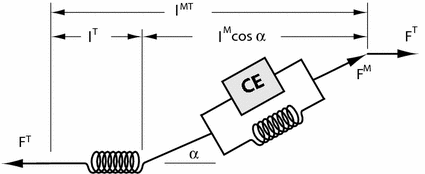
\includegraphics[width=8cm]{Figures/hill_type_muscle_model.png}
%  \caption{Hill muscle model \citep{Arnold2010}}
%  \label{fig:hill-model-Muscle}
%\end{figure}
%Where $F^{KT}$ and $F^{KM}$ are the spring forces of the tendon and muscle respectively, which are a function of extension length. $F^CE$ is the contractile force and $F^T$ is the total contractile force as observed at the end of each tendon either end of the muscle. Where  $F^T$ is the tendon force; $F^M$ is the muscle force; the $l^T$, $l^M$, $l^{MT}$ are muscle length, tendon length and their combined lengths respectively; $\alpha$ is the pennation angle (i.e. zero if parallel muscle); The left and right non-linear spring elements represent a tendon and muscle spring characteristic respectively; The CE box represents the contractile element that generates contractile force. 
%\begin{equation}
%    F^T = F^{KT} + (F^{CE} + F^{KM})cos(\alpha)
%    \label{eqn:hills-model}
%\end{equation}


%\subsection{Electrical Muscle Stimulation and Models}
Similar to EAP-based artificial skin and artificial muscles, biological muscles also require electrical stimulation in the form of neuronal action potentials to function. These models often require many input parameters to determine the out contraction force and strain of a muscle such as action potential frequency, nerve conduction velocity, calcium ion absorption dynamics, and concentrations of many other molecules required in the process \cite{Purves2001}. In contrast, when designing artificial muscle technology there is opportunity to control the parameters for their electromechanical models.
%
%For an artificial electrical stimulation to a muscle, 
%
%to simulate the signal a motor neuron would give to a muscle, is functional electrical stimulation (FES). Due to the biochemical nature of the motor neuron signal transport and the purely electrical stimulation provided by the FES device, the process isn't as efficient as the naturally occurring electro-chemical muscle activation, often resulting in increased muscle fatigue when compared to equivalent voluntary muscle contractions \citep{Ibitoye2016}. FES applies a voltage across between two electrodes on the user's skin above a specific muscle. The voltage simulates the signal form and frequency of action potentials between 4 - 12Hz \citep{Popovic2004}. The threshold for a muscle action potential to cause a muscle contraction is approximately  mV \cite{}.
%%\begin{figure}[H]
%%  \centering
%%  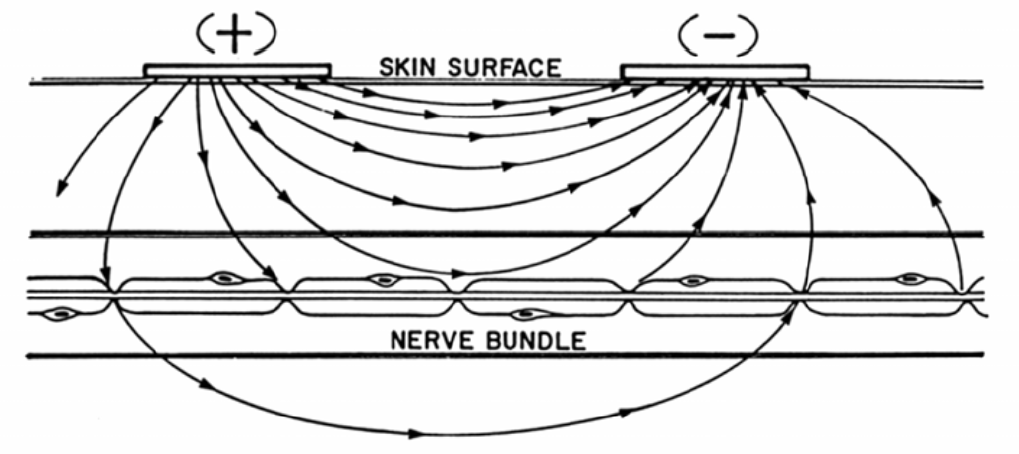
\includegraphics[width=8cm]{Figures/FES_electric_field.PNG}
%%  \caption{Electric field generated by two electrodes on the surface of the skin above a specific muscle and hence it's activating nerve bundle \citep{Bajd2010}}
%%  \label{fig:Muscle}
%%\end{figure}
%To artificially sense an intended muscle contraction electromyography (EMG) can be used. EMG also commonly uses two electrodes on the surface of the skin above a desired muscle. This EMG signal can be used as a sensor input for joint pose estimation. EMG senses the action potential impulses conducted along motor neurons to the muscle. 
%There are many models for limb motion and EMG- and FES-based therapies \cite{Meadmore2014,Freeman2015,Hodkin2018,Popovic2014}.




\section{Artificial Actuation - Electromagnetic Actuator Technology}
\label{sec:Artificial Actuation - Electromagnetic Actuator Technology}
Artificial muscle actuator technology has been refined over the course of the 21st century to more closely match biological muscle and supersede them in certain performance metrics. The most prominent soft actuator technologies researched in recent years include, ionic polymer-metal composite (IPMC) actuators, hydraulically amplified self‐healing electrostatic (HASEL) actuators, magnetorheolgical elastomer (MRE) actuators, and dielectric elastomer actuators (DEAs). Each of these having qualities similar to that of biological muscle usually with a trade-off in actuation response time, actuation force, and actuation strain for their various possible topologies. This section gives a brief overview of four state-of-art soft EAP actuator technologies.

\subsection{Current Driven - Ionic polymer–metal composite actuator}
Ionic polymer-metal composite actuators (IPMCs) are soft actuators that can be actuated at a much lower excitation voltage than DEAs, commonly less than 10V. IPMCs are also desirable as artificial muscles they have shown large bending deformations, simple to fabricate, light weight and thin in design, and can have a fast actuation response time ($>$ 15 Hz) at small displacements \citep{Ma2020}. IPMCs also have a high work density and maintain a constant volume during actuation like biological muscles \cite{Neuhaus2020}.
\begin{figure}[H]
  \centering
  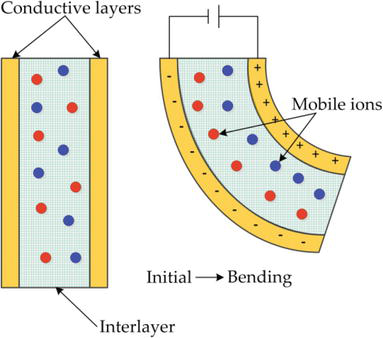
\includegraphics[width=0.5\linewidth]{Figures/IPMC.png}
  \caption{Diagram of the typical architecture of an IPMC actuator \citep{Wang2018} ($\copyright$ 2018 Yanjie Wang and Takushi Sugino)}
  \label{fig:Artificial Muscle_IPMC}
\end{figure}
An IPMC is made up of an ionic polymer inter-layer, two electrode conductive layers, and a voltage source. The ionic polymer inter-layer allows for ionic transport and is typically made of treated Nafion or Flemion. These materials are typically used as ion exchange membranes so have the characteristics desired for the transporting ions during the actuation of the IPMC actuator. The two electrodes are made of a suitably conductive and flexible material. The inter-layer is treated such that it is filled with water molecules and cations, with the chemical backbone of the inter-layer being slightly negatively charged. When a voltage is applied across the electrodes the cations are repelled from the cathode and travel towards the anode while the water molecules are displaced in the opposite direction towards the cathode. The ionic polymer then swells as the cations repel each other along the anode side of the inter-layer, while the polymer elements on the cathode side effectively shrink \citep{Segalman1999}. This swelling adjacent to the cathode provides the device's bending actuation.

There are many variations of the design and manufacturing of IPMCs to optimise the actuator for an application as shown by \cite{Shahinpoor2016}.

Although the process of manufacturing IPMCs is simple, the typical duration for the ionic polymer to absorb the necessary ions and undergo necessary reaction during fabrication can exceed 48 hours \cite{Ma2020a}. There has been much research into the optimal manufacturing of an IPMC \citep{Homma1999,Liu1992,Shahinpoor2016}. The use of additive manufacturing has been used successfully to generate more complex geometries using fused filament deposition \citep{Carrico2015}.

IPMCs can also be used as sensors. When an IPMC undergoes bending due to an external force there is a potential generated across the electrodes, which indicates bending direction and magnitude \citep{Shahinpoor2004}.

Two key deficiencies of current IPMC actuator technology are the maximum force output achievable and the life cycle of the actuator in a dry (non-aqueous) environment. The force output optimisation of IPMCs has been investigated by several researchers, all of which having a maximum actuation force in the milli-newton scale \citep{Akle2004,Xu2014,Shahinpoor2004}. Because the IPMC actuators rely on hydrated ionic transport to actuate this means if the IPMCs are in a dry environment then over time they will decrease their maximum actuation force.

The applications of this actuator is limited to applications requiring a small actuation force and a wet environment. Some current applications include flexible catheters \citep{Guo1994}, small biomimetic robotics \citep{Kodaira2019,Chang2013}, and aquatic robotics \citep{Hubbard2014,Khawwaf2019}.


\subsection{Magnetically Driven - Magnetorheological Elastomer}
Magnetorheological elastomer (MRE) actuators, also known as magnetoactive soft materials (MSMs), are a relatively new form of actuator however the theory reinforcing operating principle has been known since at least the 1980s \citep{Jolly1996}. The structure of an MRE actuator generally consists of a ferromagnetic elastic composite and a driving magnetic field. An example of this is a composite of iron-carbonyl powder and PDMS. The operating principle of MREs is magnetostriction, where magnetic flux travelling through the MRE will change mechanical characteristics within the elastomer (i.e. stiffness and/or deformation of the body). The operation of a MRE actuator is similar to a DEA however instead of having an electric field cause a contraction it is a magnetic field causing a deformation. An MRE is typically made of silicone rubber containing magnetic ferrite based particles uniformly distributing throughout its volume. This kind of actuator is current controlled and can hence operate at a low voltage. This helps mitigate the risk of electric shock of a device in close proximity to humans, unlike HASEL and DE actuators discussed in the following Sections \ref{subsec:hasel-actuator} and \ref{subsec:DEA}.
\begin{figure}[H]
  \centering
  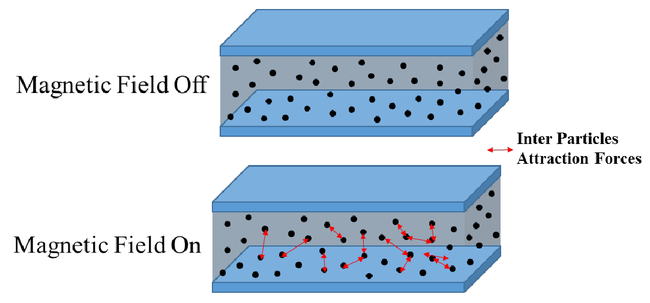
\includegraphics[width=0.6\linewidth]{Figures/MRE_actuate.jpg} %%% TO DO: get permission from Author!!
  \caption{Diagram showing MRE contraction forces when a magnetic field is applied \citep{Park2018a} ($\copyright$ 2018 Yu-Jin Park et al. | SPIE).}
  \label{fig:Artificial Muscle_MRE}
\end{figure}
A key issue with using magnetorheological elastomers as soft actuators is that they require heavy gauge conductors for the high current they require for generating a magnetic field. The high current requirement means that actuators have only been created that have a rigid electromagnet driving a soft MRE \citep{Bose2012}. 

When manufacturing MREs, uncured liquid silicone rubber is mixed with magnetic (commonly carbonyl iron) particles to form a 3D matrix of cross-linked elastomer with homogeneously dispersed magnetic particles. A core issue when creating an MRE is the agglomeration and corrosion of magnetic particles due to residual water within the mixing operation. The magnetic particles can be processed to have a hydrophobic quality to mitigate this issue \cite{Burhannuddin2020,Ge2020}. During the curing process a magnetic field can be applied to align the particles within the elastomer to control the particle isotropy \cite{Ge2020,LaleganiDezaki2023}.

There have been attempts to use additive manufacturing to make MREs \citep{Krueger2014,Ge2020}, however the method described has not optimised the structure of MRE for any application and the particle dispersion throughout the MRE has not been proven uniform throughout the print volume. 

To sense the contraction and deformation of an MRE a hybrid iron-carbon particle elastomer composite can be made. Where the carbon particles' contribute to the material piezoresistivity to determine the material loading \cite{Bica2011,Costi2024}. 

The current applications of MRE actuators are limited, however magnetorheological fluid (MRF), is a fluid which becomes more viscous with an applied magnetic field as currently has many modern applications. This fluid substance is largely used in applications where damping control is desired such as vehicle suspension \citep{UnuhH2019}, medical assistive devices \citep{Chen2017} and helicopter seat damping \citep{Hiemenz2007}. Potential MRE actuator applications include fluid valve control \citep{Bose2012} and active vibration control similar to that mentioned for MRFs \citep{UnuhH2019}. 


\subsection{Electrostatically Driven - HASEL actuator}
\label{subsec:hasel-actuator}
A hydraulically amplified self‐healing electrostatic (HASEL) actuator is a recent soft actuator technology developed in 2018 by Kellaris et al.\citep{Kellaris2018} which displays many qualities that are superior than current artificial muscle technology. HASEL actuators are made up of three main components: electrodes, dielectric fluid, and an elastomeric shell. The electrodes need to be highly conductive, able to handle high electric potential, and can be solid or flexible. Hydrogel electrodes have been proven to be a good material for the electrodes because of their elasticity while still maintaining a high conductivity \citep{Acome2018}. In one application the hydrogel material is bonded to a polydimethylsiloxane (PDMS) substrate for mechanical strength and for ease of bonding to the actuator bi-axially-oriented polypropylene (BOPP) shell \citep{Kellaris2018,Yuk2016}. HASEL actuators use high electric potential across two electrodes to create an electrostatic force. This force induces a zipping effect which pulls the electrode together from one end to the other as the electric field strength increases. The zipping of the two electrodes pushes the dielectric fluid into the reservoir increasing the pressure which alters the shape of the reservoir bounds providing an actuation motion. When the electrodes have displaced all of the fluid between them the actuation displacement is at a maximum. The electrostatic zipping action allows a large force to be generated due to snap-through transition. Snap-through transition is an actuation instability which has been discussed in previous research as a means of amplifying DEA actuation strain \citep{Keplinger2012}. 
\begin{figure}[H]
	\centering
	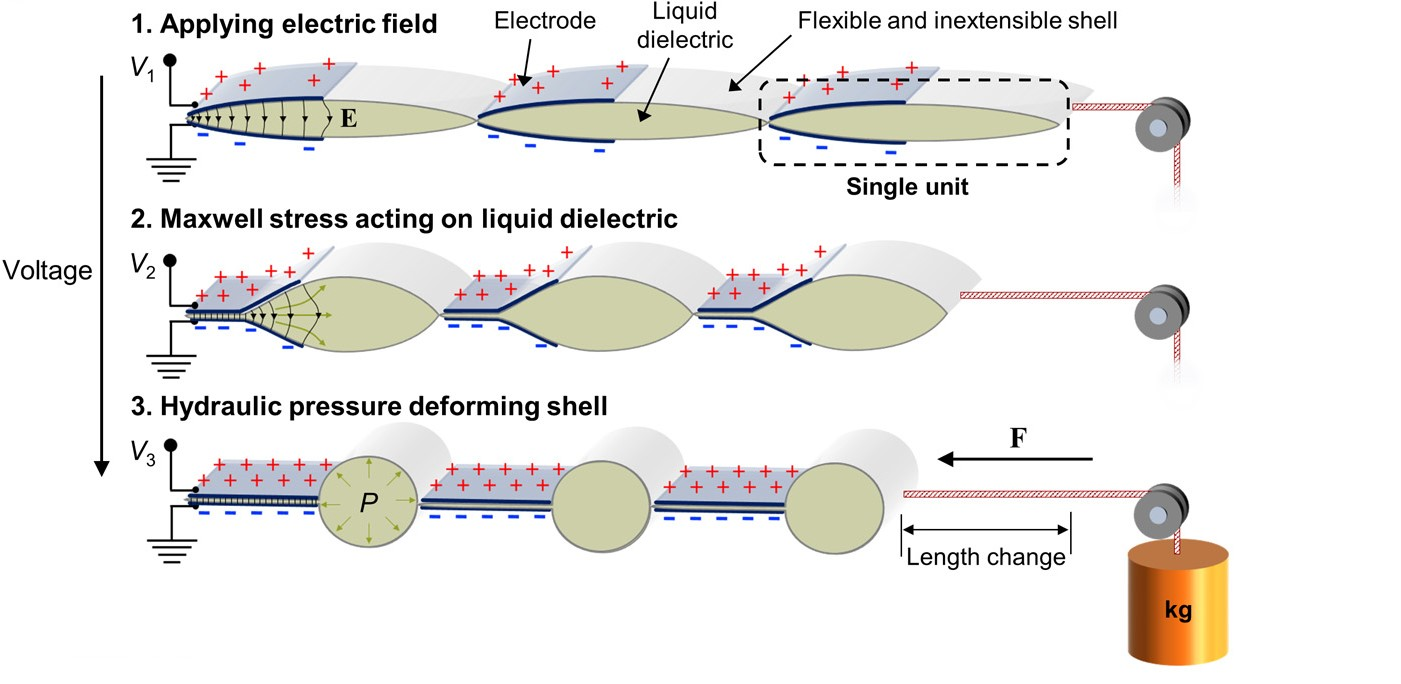
\includegraphics[width=0.7\linewidth]{Figures/HASEL_actuator_crop.jpg}
	\caption{Diagram of the typical architecture and the contraction stages of a HASEL actuator \citep{Kellaris2018} ($\copyright$ 2018 Nicholas Kellaris et al. | AAAS).}
	\label{fig:Artificial Muscle_HASEL}
\end{figure}
Recorded efficiency values of HASEL actuators of 21\% are comparable to that of human muscles of 20 - 35\% \citep{Smith2005}. The actuators have had a frequency response of up to 20Hz. Large strains of 124\% have been recorded, but can only be achieved when actuating at a resonant frequency. Strains of up to 79\% have been recorded using a linear planar HASEL actuator configuration and DC voltage stepping.  Else, strains of only 10\% have been recorded for static steady strain \citep{Kellaris2018}.
Because there is a relationship between the motion of the actuation and capacitance between the electrodes, this means self sensing can be achieved through the electrodes. Although due to the flexible and fluid nature of the device, modelling of the HASEL is difficult and limited in accuracy.

The simple and commonly used manufacturing process for HASEL actuators is completed in six steps as shown by the diagram below:
\begin{figure}[H]
	\centering
	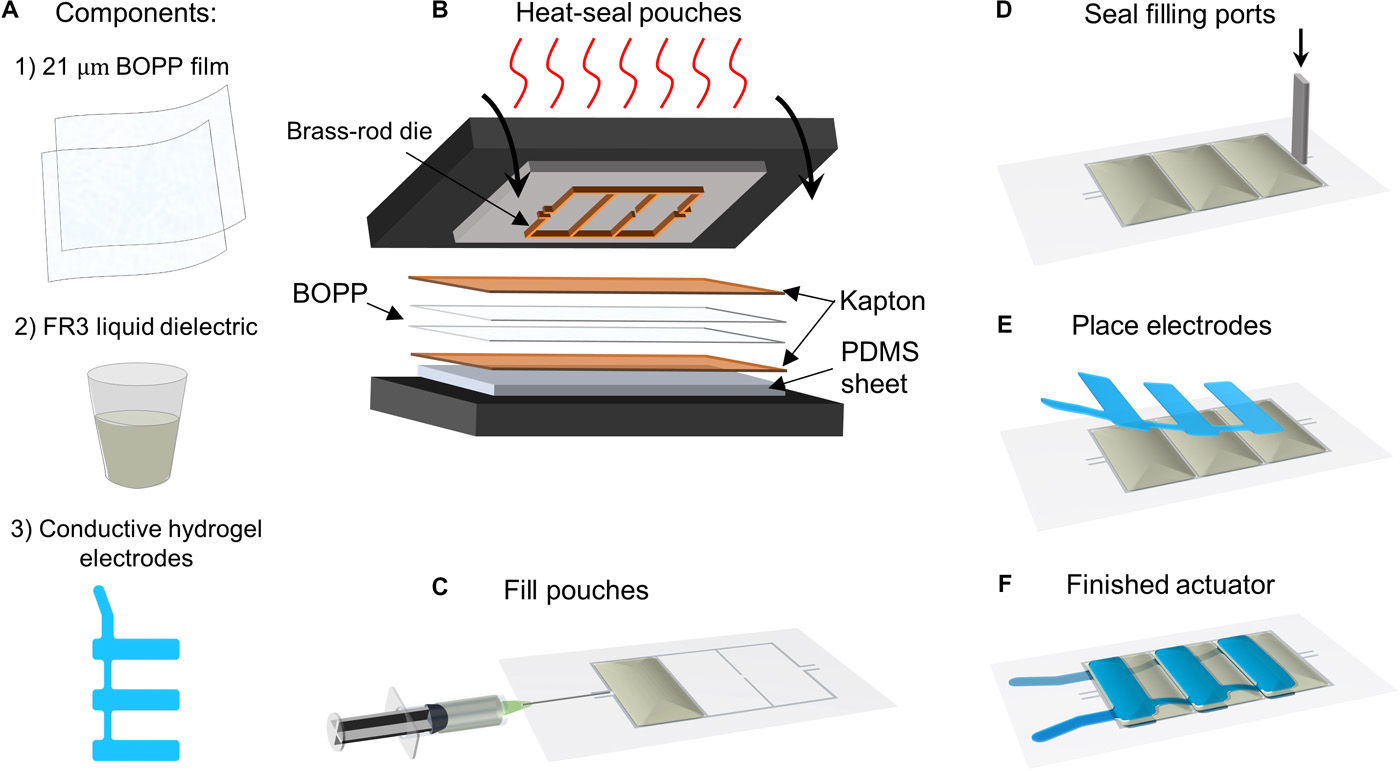
\includegraphics[width=0.7\linewidth]{Figures/HASEL_manuf.jpg}
	\caption{Diagram of the simplified stages of HASEL actuator production \citep{Kellaris2018} ($\copyright$ 2018 Nicholas Kellaris et al. | AAAS).}
	\label{fig:Artificial Muscle_HASEL_manf}
\end{figure}

Other attempts have been made to use polyjet inkjet based additive manufacturing to make the whole HASEL actuator and have been successful with proof of concept, but are yet to be developed from prototype stage \citep{Manionn.d.}. 

The cyclic life of HASEL actuators are high, because of their self-healing properties. When there is a dielectric breakdown through the liquid dielectric the damage caused is not permanent like when a DE breaks down. The liquid may form some small air bubbles, however these may not effect the operation of the actuator, instead this can increase the likelihood of a another dielectric breakdown. The cycle life of the HASEL actuator was seen to be larger than one million with a given torus shaped HASEL actuator \citep{Acome2018}. The HASEL technology is promising with a number topologies possible,  including toroidal, planar linear \citep{Acome2018}, and scorpion metasoma(tail) \citep{Mitchell2019}.


\subsection{Electrostatically Driven - Dielectric Elastomer Actuators}
\label{subsec:DEA}
% How do DEAs work
DEAs share many similar characteristics to biological muscle such as, the large strains achievable, the high elastic energy density, many topologies/configurations achievable, and constant volume during its contraction. Compared to the previous soft actuator technologies discussed, the dielectric elastomer actuator (DEA) better fits the term `artificial muscle'. 

A DEA consists of a dielectric elastomer (DE) film sandwiched between two compliant electrodes. To excite the actuation, a high electric potential is applied to across the electrodes creating an electrostatic force between the two compliant electrodes. This force pulls the two electrodes together applying stress (known as Maxwell's stress) to the elastomer and hence strain parallel and perpendicular to direction of the electrostatic force. When the DEA is contracted the surface area of the electrodes increases and the thickness of the DE decreases causing a change in capacitance and Maxwell's stress.
\begin{figure}[H]
	\centering
	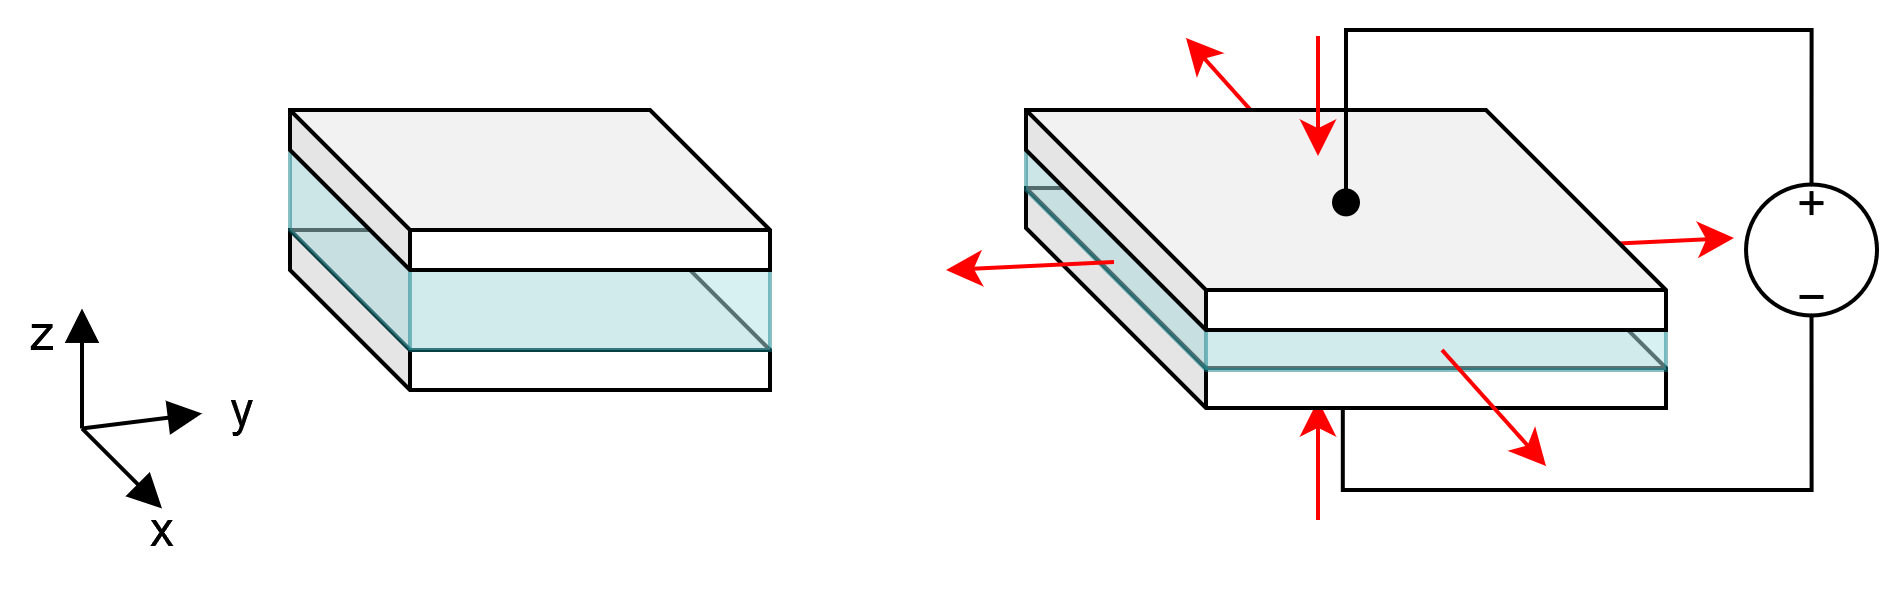
\includegraphics[width=0.7\linewidth]{Figures/dea_square_2state.jpg}
	\caption{DEA with two compliant light-grey electrodes and a transparent light blue dielectric elastomer. Showing deformation without and with a voltage applied across the electrodes.}
	\label{fig:Artificial Muscle_DEA}
\end{figure}
A dielectric elastomer actuator can be modelled as a flexible parallel plate capacitor in its simplest form. Using this we can determine the electrostatic pressure to be:
\begin{equation}
	\sigma_{es} = \epsilon_0 \epsilon_r \frac{V^2}{z^2}
\end{equation}
Where $\sigma_{es}$ is the electrostatic pressure, $\epsilon_0$ and $\epsilon_r$ are the vacuum and relative permittivity constants, $V$ is the voltage potential applied across the electrodes and $z$ is the thickness of the DE. The electrodes used for a DEA need to be made of a conductive material, but require similar elasticity to the dielectric material. An ideal material for these electrodes would have high conductivity. This conductivity would change minimally and predicatively under large strains. Many composites have been used in practice for these electrodes, with the most common in early development being a silicone rubber and carbon powder composite or a carbon grease. However, the unpredictable nature of carbon powder elastomer composites has lead to research into many other materials/silicone additives such as hydrogels, graphene sheets, metallic nanostructures, carbon nanotubes, liquid metal \citep{Liu2013,Rogers2013,Bele2018,Quinsaat2015}. The ideal material for the dielectric elastomer should have a high elastic modulus and a high electric breakdown voltage. The elastic modulus needs to be sufficiently low so that less electrostatic pressure can create a larger strain. The actuation force is also a function of the dielectric constant, with increased dielectric constant resulting in increased actuator force.  

While the breakdown voltage of the material needs to be sufficiently high such that the material will not break down at the maximum desired strain. If a material can be found with a high enough electric breakdown strength at a smaller thickness than current research prototypes then a higher stress can be achieved giving a larger or equivalent actuation force at a lower voltage. 

While disc shaped DEAs are the most commonly used actuator topology many other topologies exist to generate different actuation motions using the same electrostatic pressure generation principle. These include actuator topologies such as stack \citep{Hau2018,Kovacs2009}, helical \citep{Carpi2012}, bending \citep{Pfeil2020}, lens \citep{Ghilardi2019}, cylindrical, and rolled shaped actuators \citep{Amin2018}. Each of which having a range of applications.

DEAs are often fabricated in a laboratory environment using a pre-strained elastomer. The pre-straining accomplishes four key qualities; stores elastic strain energy, ensures DE is planar within the bounds of the jig, controls the initial thickness of the DE, and puts the DE in an optimal stress-strain region, often taking advantage of elastomer hyper-elasticity. There is no standard practice for the fabrication of DEAs, other methods such as additive manufacturing have also been explored to generate more complex geometries and to increase production speed \citep{Park2018,McCoul2017}.

As well as actuating, DEAs can also be used for sensing. DEAs can be used as sensitive capacitive sensors, where any strain applied to the DE will relate to the effective capacitance between the two electrodes \citep{Jung2008,Goulbourne2007,Gisby2013}. 

Currently DEAs often require voltages within the kilo-volt range to generate an adequate stress and strain for a range of applications. A key problem encountered by researchers designing DEAs is the trade-off between actuation force and strain magnitude \citep{Hau2018}. This high voltage requirement may deem the technology dangerous for use where there is a possibility that a human may come into physical contact with the high voltage electrodes.


\section{Electroactive Material - Soft Conductive Particle Piezoresistive Composites}
\label{sec:Soft Piezoresistive Composites}
% Why are soft piezo resistive composites used in S&As?
Most soft sensors and actuators require low-stiffness materials for their active sensing/actuation domains. The requirement of softness is governed by the mechanical modulus values depend on the application requirements. The use of conductive particle elastomer composites is explored in this work due to the customisability of the electromechanical characteristics. Although HASEL actuators have been defined soft actuators they commonly BOPP or BOPP-like plastic polymers which are flexible, however do not have the desired stretchability of elastomers. When comparing the limited amount of relatively soft piezoresistive materials in comparison Table \ref{tab:comparing-piezo-r-materials}, conductive particle polymers were determined to have the best fit for the sensor and actuator technology developed in this work.
% Why CPECs
A core part of this thesis is understanding the behaviour of conductive particle elastomer composites for their use as a range of EAP-based sensing and actuating devices. The characteristics that make conductive particle elastomer composites (CPECs) ideal for soft sensor and actuator devices often include, its customisable low stiffness, conductivity, piezoresistivity, elasticity, mouldability,  as well as its 3D printability, low toxicity, durability, cost, simple fabrication process, and sustainability \cite{Chung2020,Ge2020,HindermannBischoff2001,Kim2012}.


\subsection{Conductive Particle Elastomer Conduction Mechanisms}
Depending on the fabrication process stages stated in Section \ref{subsec:Fabricating Conductive Particle Elastomer Composites} for fabricating CPECs, the dispersion of conductive particles will always vary. 

\begin{figure}[H]
    \centering
    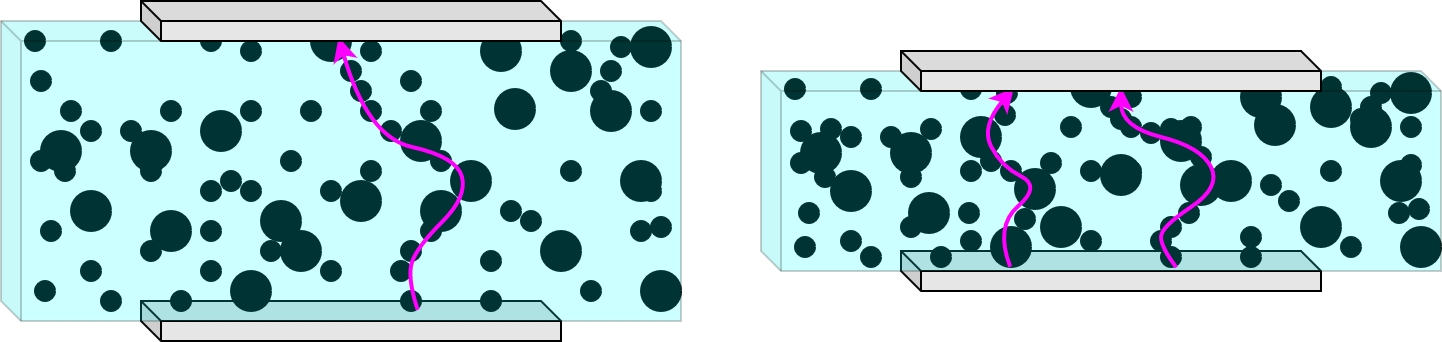
\includegraphics[width=0.7\linewidth]{Figures/res_deformed_states_x2_crop.jpg}
    \caption{Two grey highly conductive electrodes across a CPEC cuboid showing enlarged black conductive particles within a blue polymer matrix. Left: An uncompressed CPEC. Right: A compressed CPEC.}
    \label{fig:res_deformed_cube}
\end{figure}

Derived from percolation theory \cite{Spahr2017}, there is a percolation threshold volume percentage of CB required for there to be a high likelihood that there is a conductive link of CB particles between two sides of a volume. Some of the physical features of these conductive percolation networks can be quantified and directly relate to the macro-level electromechanical properties of the material. Such characteristics of a conductive percolation network include, the type of conductive particle(s) used, particle dispersion, the elastomeric matrix, and any impurities or voids. The aspect ratio of a conductive particle filler can drastically change the conductivity and piezoresistivity of a CPEC. For example the aspect ratio of carbon nanotube particles (CNTs) is very large compared to that of regular carbon black (CB) particles, this has been shown to give improved conductivity for smaller weight/volume percentages \cite{Wu2019,Flandin1999}, among other electromechanical property changes. Also the inherent particle conductivity a core parameter to consider when choosing a conductive particle composite. An example percolation threshold plot is shown in Figure \ref{fig:perc-thresh-plot}.

\begin{figure}[H]
	\centering
	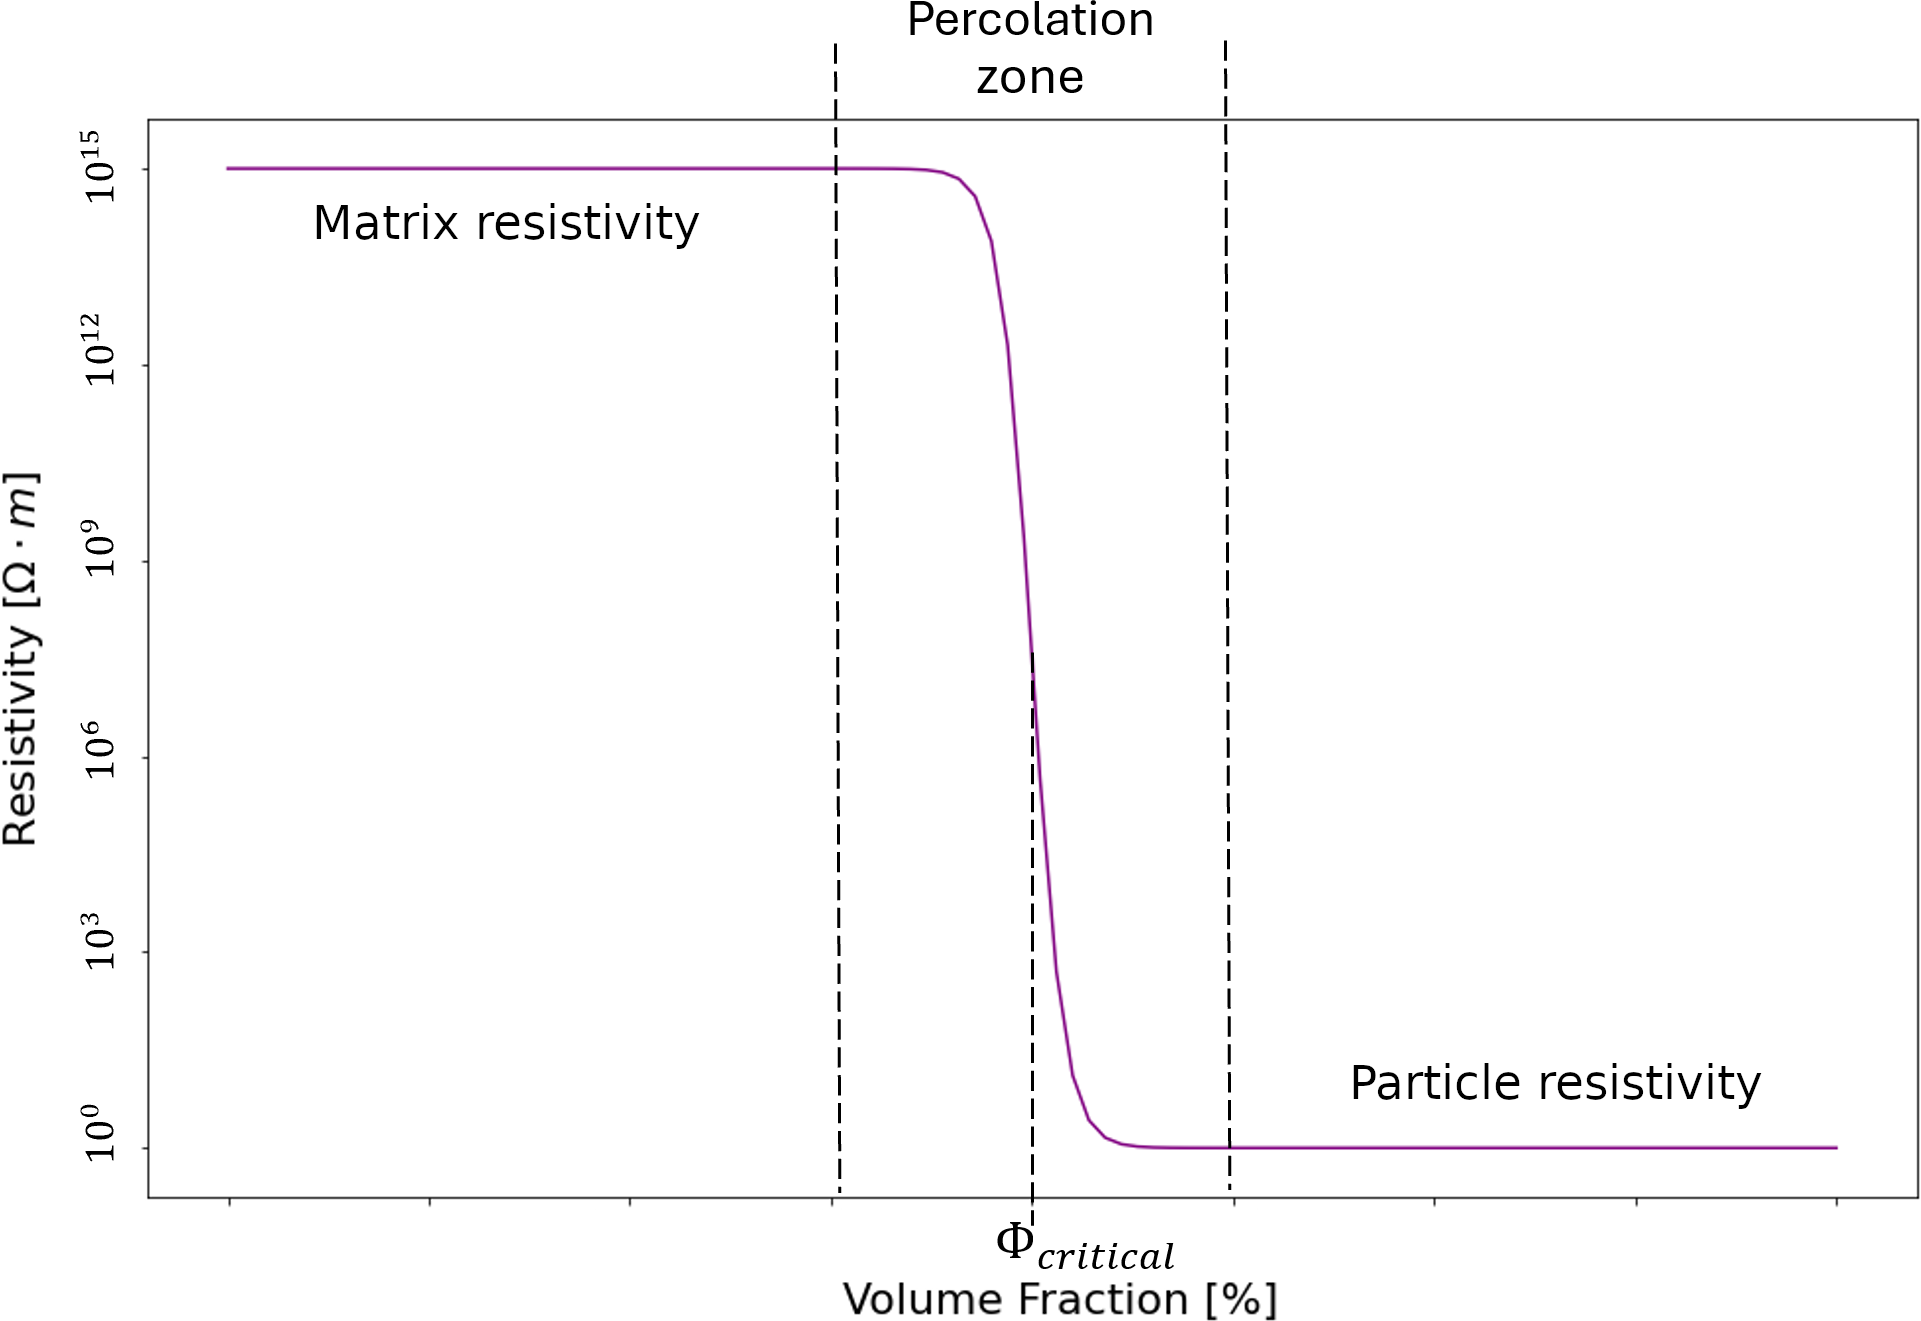
\includegraphics[width=0.7\linewidth]{Figures/percolation-plot-example_labelled.png}
	\caption{Example percolation threshold plot for a conductive particle composite with the plot settling at the conductive particle resistivity.}
	\label{fig:perc-thresh-plot}
\end{figure}

Conductive particle dispersion is an important characteristic of CPECs when optimising the electrical properties of a CPEC. Particle dispersion includes the inter-particle distance distribution \cite{Kim2012}, particle agglomeration distribution \cite{Pegel2008}, particle isotropy/anisotropy \cite{Song2022}, and sedimentation \cite{Eklund2019}. The filler elastomer matrix also contributes to the piezoresistive effect, through it's viscoelasticity, elastic modulus, and dielectric permittivity within the CPEC.
% To do: Mention voids and impurities?

\begin{figure}[H]
    \centering
    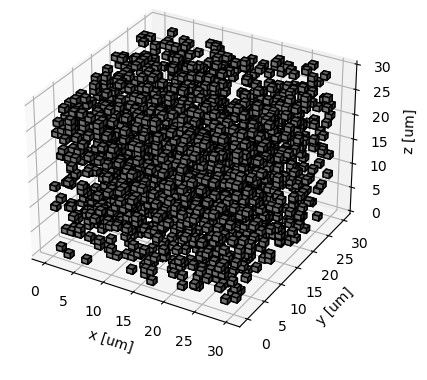
\includegraphics[width=0.6\linewidth]{Figures/simple_random_percolation.jpg}
    \caption{Example of a randomised cube percolation with a volume percentage of 8\% of 1$\mu$m particles}
    \label{fig:simp_rand_perc}
\end{figure}

% How you can model CBSR type material and the conduction mechanisms
Microscale models for CPECs and the relationship between particle and electric charge motion are often computationally heavy, overly idealised, and non-invertible \cite{Wang2022}. A microscale model example can be seen in Figure \ref{fig:simp_rand_perc}. However, microscale modelling of CPECs may give insight into understanding complex physical phenomena that may relate to the macroscale models made for CPECs. An alternate method for modelling CPECs is the formation of macroscale models \cite{Neffati2019}.
\begin{figure}[H]
	\centering
	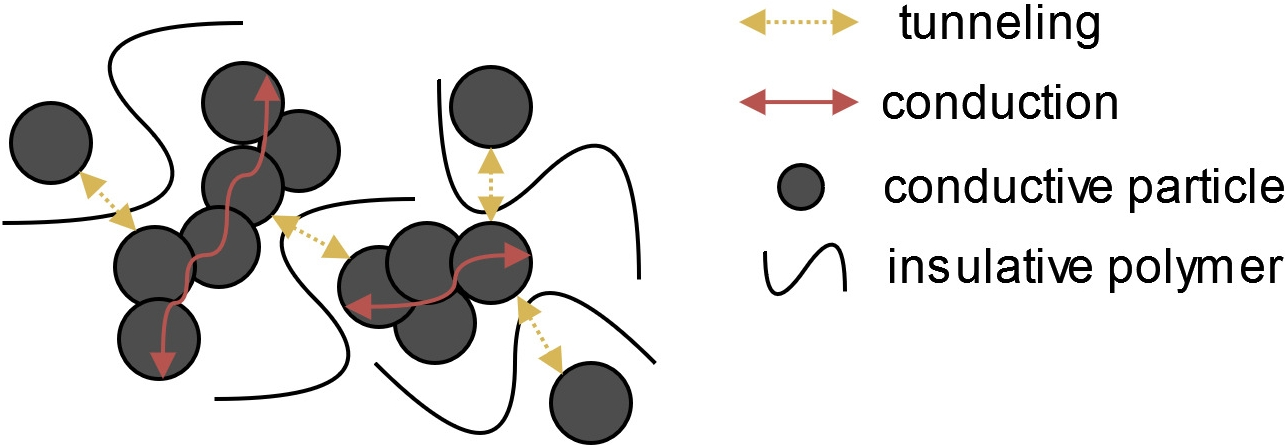
\includegraphics[width=0.7\linewidth]{Figures/conduction-tunneling-mechanisms.jpg}
	\caption{Electrical conduction and tunnelling representation diagram.}
	\label{fig:tunneling-model-rep}
\end{figure}
Electrical DC conduction through a CPEC occurs via two main mechanisms, electrical conduction and quantum tunnelling \cite{Bloor2006,Duan2014,Zhang2007,Madrid2017}. Electrical conduction uses the conduction band electrons shared by adjacent atoms to allow movement of electrons throughout chains of cascading these conductive atoms. The second mechanism of conduction is through quantum tunnelling which is stochastic in nature and allows for conduction through insulative boundaries between the percolative network of conductive particles \cite{Hu2008,Grimaldi2006}. 
\begin{figure}[H]
	\centering
	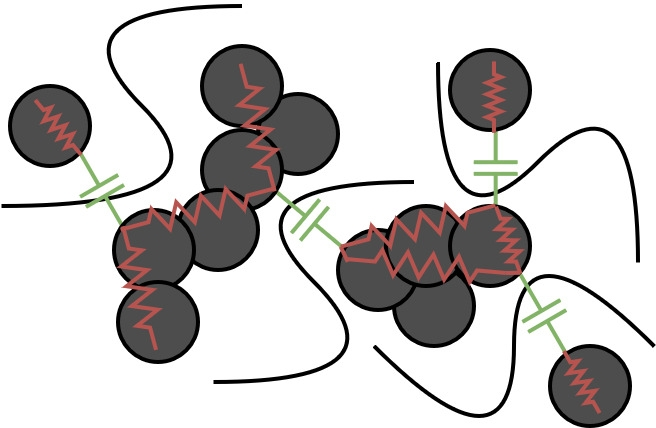
\includegraphics[width=0.4\linewidth]{Figures/conduction-AC-mechanisms.jpg}
	\caption{AC conduction RC network representation diagram.}
	\label{fig:AC-model-rep}
\end{figure}
The a CPEC can be modelled with an RC network as shown in Figure \ref{fig:AC-model-rep}. Electrical AC conduction can occur through a CPEC through capacitive means depending of particle spacing with a decrease in reactance becoming more prominent for composites near the percolation threshold \cite{HindermannBischoff2001,Ilgaz2021,Buketov2020}.


\subsection{Fabricating Conductive Particle Elastomer Composites}
\label{subsec:Fabricating Conductive Particle Elastomer Composites}
Before exploring the known conduction and piezoresistive mechanisms and models for CPECs, it is important to understand how the fabrication process of a CPEC may affect its physical structure. 

CPECs are made by dispersing conductive particles through a curable liquid elastomer matrix. To change the electromechanical properties of the material, the dispersion of the conductive particles throughout the matrix can be optimised through various methods such as mixture sonication, and mix speed and timing. Sonication serves to minimise the agglomerations of primary conductive particles as a preliminary step. This involves a mixture of the conductive particles and a liquid, usually in the form of a solvent, to be placed in a ultra-sonication bath. 

The sonication bath performs a frequency sweep and it has been shown that sudden implosion cavitation near the agglomerates help cause the separation of the agglomerates into their primary particles \cite{Priyadarshi2021,Kudryashova2019}. The degree of deagglomeration and dispersion is affected by various factors including sonication time, frequency of oscillations, oscillation intensity, particle wettability, and liquid matrix viscosity \cite{Kudryashova2019,Chen2020a}. 

This sonication usually occurs before the the particles and solvent are added to the elastomeric matrix due to the large viscous damping effects of liquid elastomers. The next step involves mixing the dispersed conductive particles throughout the liquid elastomer, this can be done using a variety of mixing methods, including a planetary mixer, magnetic mixer, screw mixer, static mixers, amongst others \cite{Pegel2008,Rosset2016,Fekiri2020,Kim2012}. During the mixing process often the liquid solvent used in the dispersion stage is evaporated, leaving only the curable elastomer and the conductive particles. Although often impurities and voids are a by-product of the previous processes which can give undesirable qualities.

When sufficient mixing of the liquid elastomer and conductive particles have been completed the material is formed into a desired final shape using advanced additive manufacturing methods \cite{Bastola2018,Sapra2023,Krueger2014,Li2020,McCoul2017,Yi2023,Park2018} or traditional moulding \cite{Kim2018} or film making techniques \cite{Fasolt2017}. During the moulding process the material undergoes a form of curing, such as UV, catalysed, or moisture curing. If the composite material has not already been integrated into a device containing electrodes and other mechanical support structures these are integrated at the end of the process.


\subsection{Viscoelasticity in Composite Elastomers}
A core difference between a pure elastomer and a composite elastomer is the degree of apparent viscoelasticity. Composite elastomers exhibit viscoelastic phenomena \cite{Ligia2009} similar to regular human biological tissue \cite{Fung1993}. These viscoelastic phenomena include strain creep, stress relaxation, hysteresis, and a strain-rate stiffness relationship. The viscous component of viscoelasticity is more prominent in polymer plastics and plastic composites due to the bonding mechanism between polymer chains within the material. Elasticity is often the result of bond stretching within a polymer material, whereas  viscous effects are often due to the temporary nature of secondary bonds in polymer which break, slip, and reform. % insert physical chemistry here!

The Payne and Mullins effects are important to note when analysing mechanical stress-strain testing results for elastomer composites with conductive filler particles. The Payne effect describes the effect where with a deformation in the material changes the modulus of the material, due to breaks in the microstructure of the material \cite{Payne1972}. Jalocha \cite{Jalocha2020} and Avila-Torrado et al. \cite{AvilaTorrado2022} have clearly displayed the Payne effect experimentally where they compared different conductive fillers and determined their complex moduli for a range of strains and strain frequencies using dynamic mechanical analysis (DMA). The Mullins effect is where the stress-strain curve of a particle filled elastomer composite relies on the maximum load input experienced by the material. The effect causes composite softening due to the lack of stiffening in the composite fillers relative to the usual stiffening seen in the elastomer matrix \cite{Mullins1969}.

\begin{figure}[H]
	\centering
	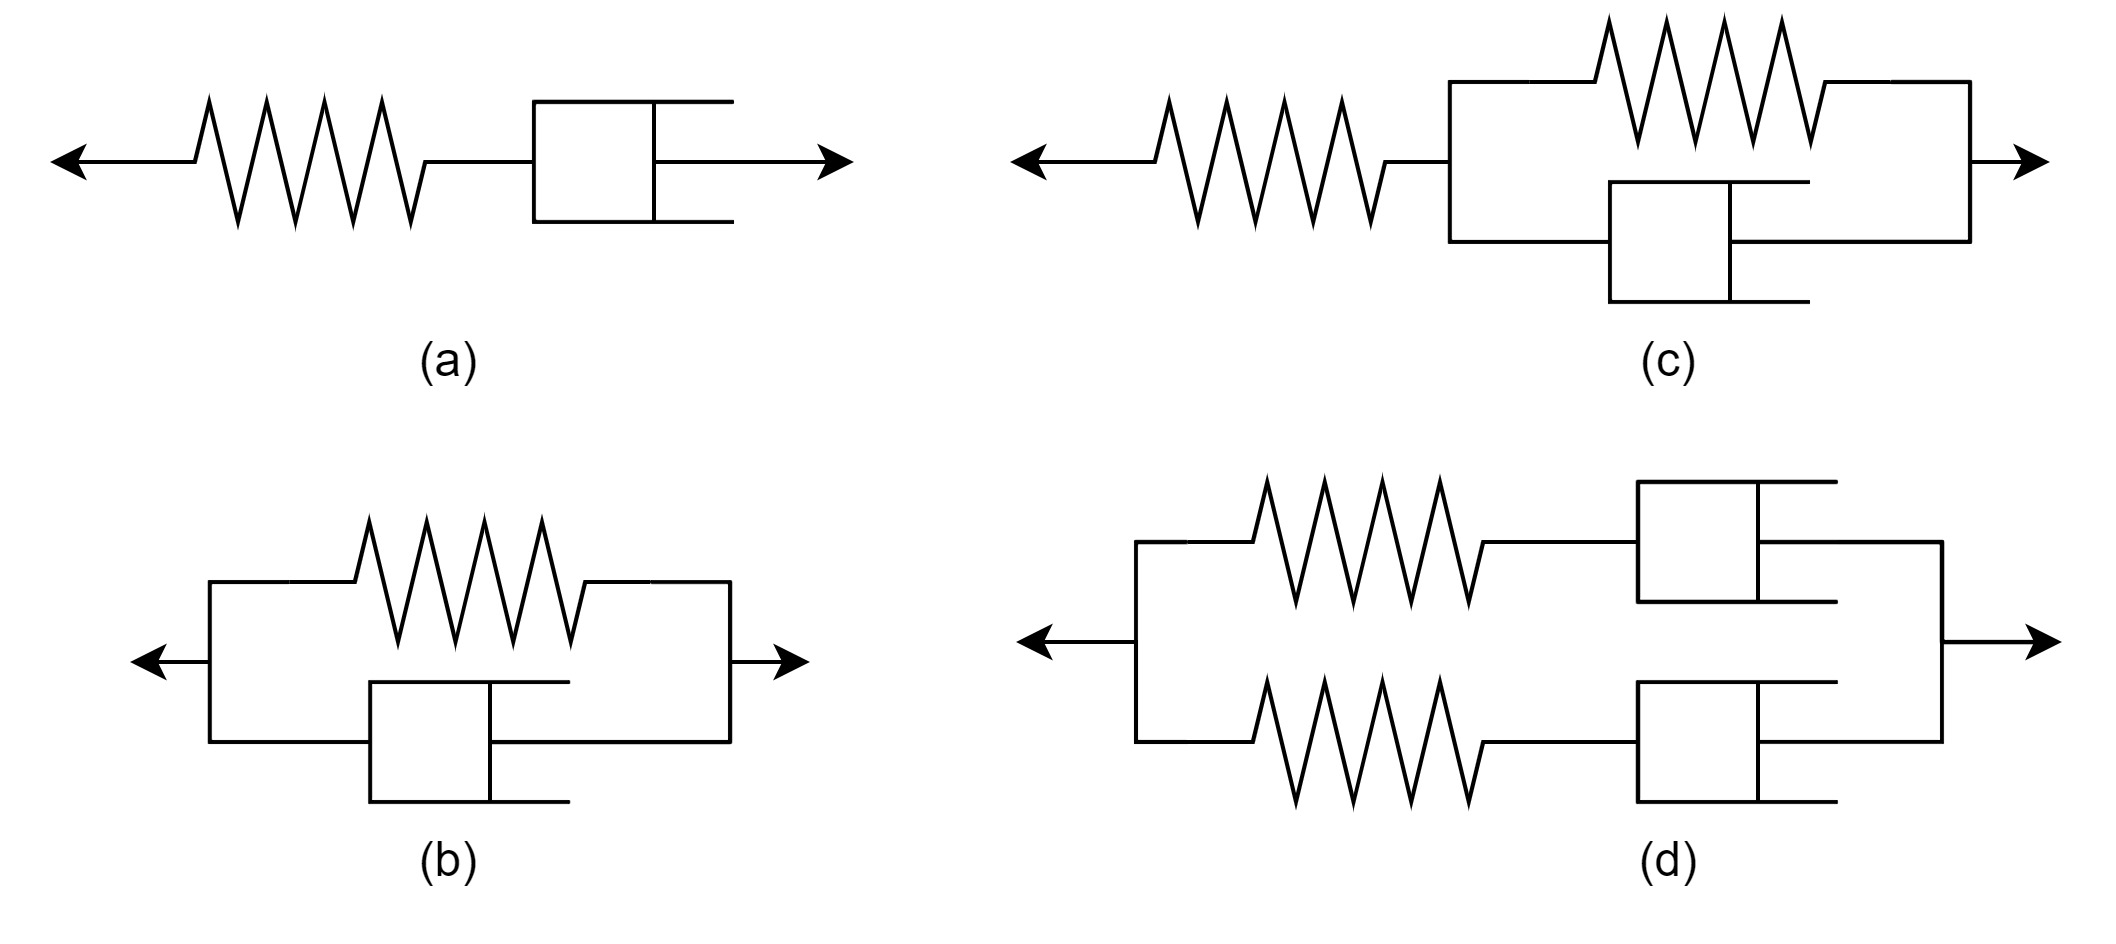
\includegraphics[width=0.6\linewidth]{Figures/viscoelastic_models.jpg}
	\caption{Linear viscoelastic models (a) Maxwell (b) Kelvin-Voight (c) A solid linear model variant (d) A Burgers model variant.}
	\label{fig:linear_viscoelastic_eg}
\end{figure}

Several linear mechanical models of viscoelastic material are described by simplifying the material to a combination of discrete spring and dashpot elements such as the Maxwell, Kelvin-Voight, Burger, and standard linear models seen in Figure \ref{fig:linear_viscoelastic_eg}. A generalised Maxwell or Prony series linear models can often be used when the other models are underfitting the material data \cite{Babaei2015,Tzikang2000}. 

Non-linear viscoelastic models are similar to the above linear models, however they introduce fractional order elements to model the complex modulus of a material more accurately \cite{Bonfanti2020}. Fractional modelling has also proven useful in complex electrical impedance modelling using constant phase elements (CPEs). These CPEs more accurately describe the non-idealness of real-world capacitors, where a current leakage through the dielectric material exists \cite{Vosika2013, Chang2022}.


\section{Soft Sensor and Actuator Technology Integration}
% Quote from lit rev intro: "The integration of soft sensing and actuation technology is reviewed and the sensor-actuator integration explored in this thesis is justified"

% To do: Throw in some lit review about the intregration of both pressure mapping and actuator devices. How has this been done in the past... if at all?

% Copy from Chapter 6??
As mentioned in Section \ref{sec:Artificial Actuation - Electromagnetic Actuator Technology} comparing electromagnetically driven actuator technology. Each of these technologies can use their active actuation area as a sensor area. IPMCs can sense bending direction and deformation with output voltage. MREs have been shown to self sense with the additional dispersion of conductive particles. HASEL and DE actuators have been shown to self sense using capacitive means. 

In this thesis the integration of a artificial skin and muscle is desired to advance the current state of soft robotic technology. To emulate this integration with current soft pressure mapping and soft actuator technology each of these actuators can be arrange in an array structure to generate pressure maps while maintaining actuation function. However, this array design introduces complications with connecting each sensel/actuation-unit and the bulk involved with wire routing and related circuitry. A more elegant solution is to maintain the active sensing and actuation area free of wires with the addition of only periodic boundary electrodes, which can be achieved using electrical impedance tomography (EIT). An EIT-based pressure mapping solution explores a piezoresistive film that can wrap around many surface topologies including adding soft actuator surfaces.

\subsection{Electrical Impedance Tomography and Pressure Mapping}
% To do: Why EIT-based pressure mapping?
% Defining EIT
To approximate changes of resistivity in a planar CPEC sensing domain a technique called electrical impedance tomography (EIT) can be used. EIT generates impedance maps for a domain under test (DUT). Unlike most pressure mapping sensors, EIT uses periodically spaced boundary electrodes to pass known electrical current and measure voltage potentials around the DUT. From these known current injections and voltage measurements, an ill-posed inverse problem can be defined. To obtain an EIT image reconstruction three key steps are required: data acquisition, forward modelling, and inverse problem solving. A constant current can be employed to capture solely the resistance values of the DUT. To capture impedance data an AC signal is implemented to sweep through a range of frequencies. 

Various electrode excitation patterns can be utilised for EIT, each with distinct reconstruction performance characteristics \citep{Russo2017,Sherry2006,Brown1987}. The most prevalent excitation pattern is the Adjacent Electrode pattern, where a current source is placed across adjacent electrodes, and the voltages at all other adjacent electrodes are measured \citep{Adler2021}. This process repeats for each pair of adjacent electrodes as exemplified in Figure \ref{fig:EIT_adj_drive}
\begin{figure}[H]
	\centering
	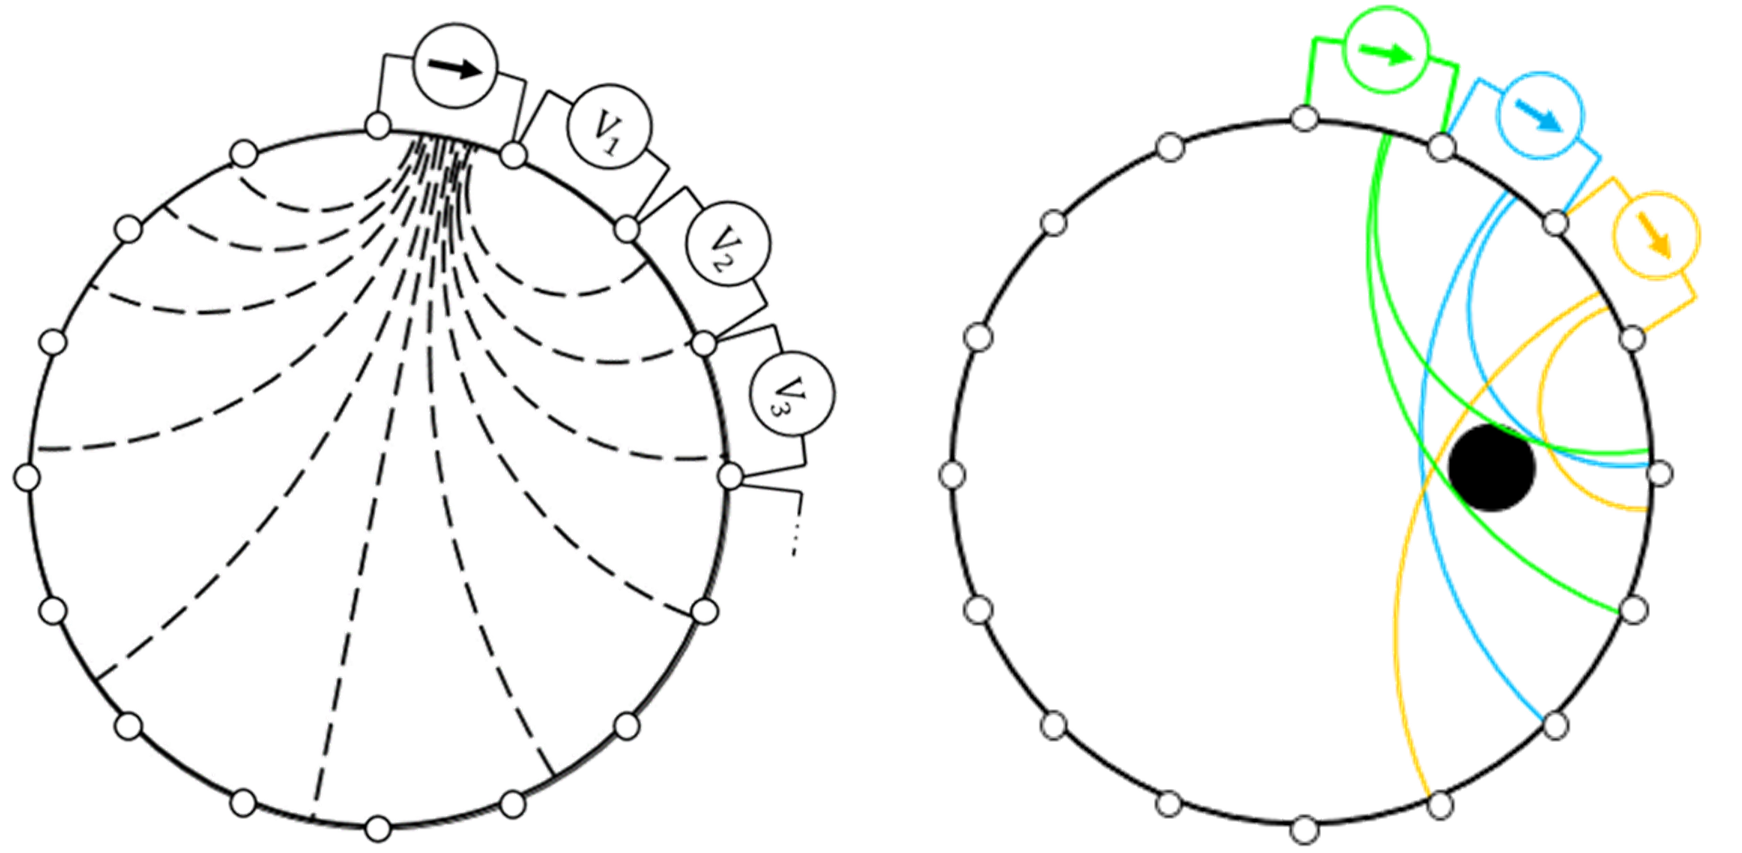
\includegraphics[width=0.8\linewidth]{Figures/eit_sequence.png}
	\caption{EIT adjacent drive pattern sequence for a circular domain with 16 boundary electrodes.}
	\label{fig:EIT_adj_drive}
\end{figure}

The forward problem in EIT is a well-posed mathematical problem, so linear algebra can be employed for obtaining electric field data for a DUT of known conductivity and a known current injection. Utilising a mesh-based coordinate system and FEM, proves to be an efficient solution for the forward model, accommodating diverse shapes. Solving the forward problem entails applying Maxwell's electromagnetic formulae and Ohm's law to determine how an electric field would propagate through the DUT, considering the DUT conductivity. voltage, $\phi$, in a domain, $\Omega$ is governed by the Equation \ref{eqn:eit-maxwells} derived from Maxwell's equations \cite{Cheney1999},
\begin{equation}
	\nabla \cdot \gamma(x,\omega) \nabla \phi = 0,
	\label{eqn:eit-maxwells}
\end{equation}
where $x$ is a point in $\Omega$ with admittivity, $\gamma$, and $\omega$ is the angular frequency of the driving current. Admittivity, $\gamma$, comprises of a real and imaginary parts $\rho(x,\omega) + i\omega\epsilon(x,\omega)$, where $\rho$ is the electric conductivity, and $\epsilon$ is the electric permittivity. Current is applied to the surface of the domain, $\delta\Omega$, through electrodes like those given in \ref{fig:EIT_adj_drive} and the current density, $J$, can be formulated with the equation
\begin{equation}
	\gamma \frac{\delta \phi}{\delta v} = J \quad on \quad \delta\Omega,
	\label{eqn:eit-current-density}
\end{equation}
where $v$ is a spatial unit restricted to the DUT boundary, $\delta\Omega$. A common continuum model used for EIT incorporates Equations \ref{eqn:eit-maxwells}, \ref{eqn:eit-current-density}, and the Law of Charge Conservation, whereby the sum of the current density and sum of the voltages on the boundary is zero. However to use these equations in practice the electrical current, $I$, is known and not current density, $J$. This is found by integrating Equation \ref{eqn:eit-current-density} for each $i$th electrode as shown in the following equation,
\begin{equation}
	\int_{e_i} \gamma \frac{\delta\phi}{\delta v} ds = I_i, \quad i = 1, 2, ..., n,
	\label{eqn:eit-current}
\end{equation}
where $e_i$ is the part of DUT boundary, $\delta\Omega$ at the $i$th electrode and $I_i$ is the current injected at the $i$th electrode. Another assumption is made with the electrode gap model when the current density between the electrodes is on $\delta\Omega$ is zero, while the current across each electrode is constant.

Unlike typical biomedical EIT imaging where there is often significant and variable electrode impedance, the device in this work uses DC meaning that no complete electrode model is needed on top of the above model constituents.

An initial estimate of the DUT resistivity is necessary for the first step of an EIT algorithm. Once the EIT forward model is solved, EIT inverse problem can be solved iteratively using the forward problem's solution. This inherently unstable problem requires optimisation algorithms and regularisation to create and linearise a solution \citep{Bayford2018,Lionheart2003,Martins2019,Adler2021}. This work uses an efficient inverse solver algorithm called Newton One-Step Error Reconstructor (NOSER) which uses a regularised form of Newton's method to solve a modified version of the inverse forward problem to generate an impedance or conductivity map based on known current and voltage values\cite{Cheney1999}. The NOSER EIT reconstruction is done via the formula
\begin{equation}
	\rho = \rho^0 C + 2 \sum_{k=1}^{K}\sum_{j=1}^{K} v_{k,j} P^{k,j},
\end{equation}
where $C$ and $P^{k,j}$ are predetermined vectors that depend only on the known geometry and regularisation parameters, and $\rho^0$ and $v^{k,j}$ are scalars determined from known data. $k$ and $j$ are the related to amount of the electrodes used and the electrode drive pattern used.
% TODO?: Insert images and equations explaining EIT??

% Explaining the required post processing
Once the EIT reconstruction algorithm has been tuned for an application, often post-processing is completed on the reconstructed EIT image for filtering and to capture data specific for the application. A consortium of experts in the field of medicine and biomedical imaging  have constructed metrics for quantifying the quality of an EIT reconstruction as shown by Adler et al. \citep{Adler2009} and their GREIT (Graz consensus Reconstruction algorithm for EIT) performance metrics. Although GREIT has been optimised for human thorax imaging, researchers who have used EIT pressure sensing purposes have also developed performance metrics, most of which agree with the GREIT metrics \citep{Silvera-Tawil2015,Visentin2016,Tallman2020,Sun2020,Hassan2009,Kato2007b}.


%\subsection{EIT-based Pressure Mapping Sensor Integration with Dielectric Elastomer Actuators}
% To do: Why DEAs? Simple construction and similar qualities to muscle.
% Why integrate? 

\newpage
\section{Literature Review Conclusions}
% Summarise: biological skin, artificial skin, biological muscle, artificial muscle, electroactive polymers.
% Clarify: the focus of the thesis.
The purpose of this thesis was to develop novel sensor and actuator technology that mimics the pressure mapping capabilities of human skin and combine this with the actuation properties of human muscle. Through this review of current literature, several key conclusions can be drawn that will lay the foundational knowledge for the rest of this work.

The review of biological skin has revealed quantitative parameters that define its mechanical and sensory capabilities. This review highlighted mechanical characteristics such as the elastic modulus, viscoelastic creep, and surface area, as well as functional properties like spatial and temporal resolution. These factors provide a foundation for designing artificial skin that can replicate or even surpass the sensing functions of soft human skin. The review on pressure mapping technologies was then completed showing a range of different transduction methods for similarly soft sensing domains, showing that replicating human mechanoreceptor sensation is a multifaceted problem. Human skin uses various mechanoreceptors with different qualities and trade-offs and similarly different pressure mapping technologies use different pressure transduction methods each with different performance characteristics and limitations. The parallel review on biological and artificial muscles showed that DEAs and HASEL actuators are promising technologies for mimicking biological muscle quantitatively. Although characteristics common to both technologies such as high actuation voltage and limited device lifetime limit the applications of them. DEAs were shown to be more akin to human muscle and skin tissue than HASEL actuators due to not only their flexibility, but their high degree stretchability, potential biocompatibility, and potential for integration with an EIT-based soft pressure mapping technology. The integration of these DEA and EIT-based pressure mapping technologies  has not yet been explored in previous literature.

The thesis has converged on using CPECs to fabricate EAP sensor and actuator devices, hence a brief literature review highlighting CPEC fabrication techniques and electromechanical characterisation has been given. These composites exhibit beneficial properties like flexibility, tunable electromechanical behaviour, and ease of fabrication, which make them suitable for integrating into soft robotic systems. However, challenges such as achieving uniform particle dispersion, minimising agglomeration, and optimising the conductive network for stable long-term operation are still active areas of investigation. Hence, this thesis first characterises some of the dynamic and time dependent properties of the material for repeated discretely categorised strain input scenarios.

The investigation of the dynamic electromechanical characteristics of CPECs and how they are used in EIT-based pressure sensors and their integration into dielectric elastomer actuators is shown in this thesis; generating technology that is more akin human muscle and skin for future integration within ubiquitous rigid robotics.
% Excite: the reader into wanting to read the rest of the thesis!

%\section{Natural World Equivalents}
%\label{sec:Natural World Equivalents?}
% Find cases where DEAs, EIT, and EFT are seen in nature! Or a VERY close analogue to really push the importance of this work.

% from ReynoldsSmith1999 -> Many species of fish use electric fields to perceive their environments. The capability has evolved independently more than once: species in two distantly related families of fish, Mormyriformes and Gymnotoidei, one from South America and one from Africa, have this capability. This split is reflected in Figure 1-1, a family tree" of the fish known to have electrosensory capabilities. The fact that electric eld sensing does not require an external light source and is unaffected by optical scatterers like mud or silt is presumably advantageous to fish in dark, murky water anywhere. Electric Field sensing is another example of convergent evolution, the best known example being the eye, which evolved independently in squid and mammals. 
%In all examples of fish electric field sensing, a current source in the tail induces voltages along the lateral line. As the sh nears an ob ject with a dielectric constant dfferent than  water, the induced voltages change. Figure 1-2 shows the electric...

%\afterpage{\blankpage}
\cleardoublepage